\documentclass[11pt]{article}
\usepackage[a4paper,margin=2.4cm]{geometry}
\usepackage[T1]{fontenc}
\usepackage{lmodern}
\usepackage{microtype}
\usepackage{amsmath,amssymb}
\usepackage{booktabs,multirow,longtable,array,tabularx}
\usepackage{xcolor}
\usepackage{graphicx}
\usepackage{tikz}
\usetikzlibrary{arrows.meta,positioning,fit,calc,shapes.misc}
\usepackage{pgfplots}
\pgfplotsset{compat=1.18}
\usepgfplotslibrary{groupplots}
\usepackage{siunitx}
\sisetup{group-separator={,},group-minimum-digits=4}
\usepackage{caption}
\captionsetup{font=small,labelfont=bf}
\usepackage{subcaption}
\usepackage{enumitem}
\setlist{itemsep=2pt,topsep=4pt}
\usepackage{listings}
\lstset{basicstyle=\ttfamily\footnotesize,breaklines=true,columns=fullflexible,frame=single,framerule=0.3pt}
\usepackage[numbers,sort&compress]{natbib}
\usepackage[colorlinks=true,linkcolor=blue!50!black,citecolor=blue!50!black,urlcolor=blue!50!black]{hyperref}
\usepackage{cleveref}
\usepackage{float}
\setlength{\emergencystretch}{3em}
\tolerance=2000

\definecolor{cstock}{RGB}{150,150,150}
\definecolor{cflash}{RGB}{196,196,186}
\definecolor{cnode}{RGB}{140,140,125}
\definecolor{cnew}{RGB}{40,110,200}
\definecolor{cbad}{RGB}{190,60,50}

\newcommand{\eVA}{\si{\electronvolt\per\angstrom}}
\newcommand{\ms}{\,ms}
\newcommand{\us}{\,\textmu s}
\newcommand{\code}[1]{{\ttfamily\def\_{\textunderscore\allowbreak}#1}}
\newcommand{\Bone}{\textbf{B1}}
\newcommand{\Btwo}{\textbf{B2}}
\newcommand{\Bthree}{\textbf{B3}}

\title{From 446\,ms to 24\,ms per Step:\\ An Exhaustive Performance Study of FP64 MACE-OFF23 Inference on a Single H100}
\author{Study report}
\date{November 2026}

\begin{document}
\maketitle

\begin{abstract}
We report a nine-phase study that reduced the latency of a complete FP64 energy+force evaluation of the MACE-OFF23 medium interatomic potential on one NVIDIA H100 from 16.3\,ms to 0.81\,ms for a 21-atom molecule and from 446\,ms to 23.9\,ms for a 5{,}184-atom periodic water box (12--20$\times$ on all supported geometries, 9$\times$ on one small-cell fallback), while staying within $1.3\times10^{-12}$\,eV/atom and $2.1\times10^{-14}$\,eV/\AA{} of stock eager FP64 MACE and reproducing its NVE energy drift. The speedup is the product of five changes, each motivated by a profile of the previous state: (1) replacing the e3nn convolution and symmetric contraction with FlashTP and cuEquivariance kernels; (2) whole-model CUDA-graph capture with padded, keyed, recapturable edge buffers; (3) two fused FP64 kernels for the edge embedding and the post-convolution node update; (4) a CUDA-graph-capturable node-centric tensor-product convolution with a single fused, atomic-free source-centric backward; and (5) a GPU cell-list neighbour builder that emits destination-sorted edges and CSR views directly, captured with the model into a GPU-resident MD step with zero host synchronisations. Along the way we found that FlashTP's FP64 mode silently rounds Clebsch--Gordan coefficients to FP32 (force errors up to $10^{-7}$\,eV/\AA{} that its own tests accept), and two silent-wrong-result hazards in naive CUDA-graph reuse. At 2{,}000+ atoms the remaining step is $\sim$99\% GPU-busy inside the model (convolution backward 27\%, radial-MLP GEMMs 25\%, elementwise 23\%). Most individual techniques are prior art (FlashTP, LunaTP, OpenEquivariance, cuEquivariance, e3j, HOOMD); we document how they compose for FP64 MACE-OFF, attribute the gain phase by phase, list more than twenty negative results, and identify the missing baselines---notably MACE's own cuEquivariance + \texttt{torch.compile} path---needed before any state-of-the-art claim.

\end{abstract}

\tableofcontents
\newpage

\section{Introduction}
\label{sec:intro}

Machine-learned interatomic potentials (MLIPs) built on $E(3)$-equivariant message passing have become the accuracy workhorse for organic and materials simulation. MACE~\cite{batatia2022mace}, and in particular the transferable organic force field MACE-OFF~\cite{kovacs2023maceoff}, sit at a favourable point on the accuracy--cost curve: two interaction layers with high body-order messages replace the deep stacks of earlier equivariant networks. Even so, a single energy+force evaluation of the stock MACE-OFF23 \emph{medium} model in double precision takes 16\,ms for a 21-atom molecule and 446\,ms for a 5{,}184-atom periodic water box on an NVIDIA H100 (\cref{sec:results}). For molecular dynamics (MD), where one wants $10^5$--$10^7$ sequential steps, that latency is the binding constraint.

This report documents a nine-phase engineering study whose goal was to make single-system, FP64 MACE-OFF23-medium inference on one H100 as fast as possible \emph{without changing its numerical result}: every optimised path was required to reproduce stock eager FP64 MACE to within $10^{-11}$\,eV/atom in energy and $10^{-11}$\,\eVA{} in force, with bitwise-identical neighbour sets. The final pipeline evaluates a complete MD step (neighbour list, forward, backward, and integration) entirely on the GPU, inside one CUDA graph, with zero host synchronisations per step. At the complete-step boundary it is 12--20$\times$ faster than stock MACE on every geometry the new neighbour builder supports, and 9$\times$ on the one small periodic cell that falls back to the older path (\cref{fig:final-speedup}).

\paragraph{What this report is and is not.}
The individual techniques are, almost without exception, known: fused tensor-product convolutions (FlashTP~\cite{lee2025flashtp}, OpenEquivariance~\cite{bharadwaj2025oeq}, cuEquivariance~\cite{cuequivariance}), destination-node (\emph{node-centric}) convolution with on-chip accumulation (LunaTP~\cite{lunatp}), CUDA-graph capture with padded edge buffers (as also used by e3j~\cite{e3j} and by MACE's own \code{compile\_mode}~\cite{mace_v0316}), and GPU cell lists (HOOMD~\cite{anderson2008hoomd}, JAX~MD~\cite{schoenholz2020jaxmd}). What we contribute is (i)~a careful, measured composition of all of them for FP64 MACE-OFF inference, (ii)~a set of correctness findings that the component libraries' own tests did not catch, (iii)~a phase-by-phase attribution of where the time went and why each step was taken, and (iv)~an honest catalogue of what did not work. We deliberately do \emph{not} claim state of the art: the strongest relevant baseline (MACE~0.3.17 with cuEquivariance and \code{torch.compile(mode="reduce-overhead")}) was available in the installed software but was not measured, and is the first experiment we recommend (\cref{sec:discussion}).

\paragraph{Contributions.}
\begin{enumerate}
  \item \textbf{A precision bug in FlashTP's FP64 mode.} Upstream FlashTP rounds its Clebsch--Gordan (CG) table to FP32 even when asked for FP64, producing $2$--$3\times10^{-9}$\,eV/atom and $3$--$10\times10^{-8}$\,\eVA{} errors against e3nn while its own test harness reports ``All Good''. We identify two independent root causes and give a 4-file, $+40/-9$ patch that restores $\sim10^{-15}$ relative agreement (\cref{sec:precision}).
  \item \textbf{A quantitative bottleneck map} of stock MACE-OFF23 inference across 3--5{,}184 atoms: a host launch floor below $\sim$650 atoms, two generic equivariant operators above it, and synchronous host-side graph construction throughout (\cref{sec:baseline}).
  \item \textbf{A safe CUDA-graph runner} for MACE with padded edge capacity, keyed graphs and recapture, including the discovery of two ``silent wrong result'' hazards (species-order reuse, 6.7\,eV/atom error; and stock FlashTP kernels escaping capture, 576\,\eVA{} error) (\cref{sec:cudagraph}).
  \item \textbf{Two fused kernels}: an FP64 edge embedding (spherical harmonics + Bessel radial basis + polynomial cutoff, forward and backward) and an algebraic per-species fold of the post-convolution linear, $1/\bar n$ normalisation and skip tensor product into one FP64 tensor-core GEMM (\cref{sec:fusion}).
  \item \textbf{A capturable node-centric FP64 convolution} with a \emph{single fused source-centric backward} that produces all three gradients without atomics; 4.2$\times$ faster than FlashTP on the L1 convolution at 648 atoms (\cref{sec:nodeconv}). The forward follows LunaTP's node-centric organisation; the capturability and the fused backward are ours.
  \item \textbf{A GPU-resident MD step}: a GPU cell-list builder that emits destination-sorted edges and both CSR views without any sort or host readback, bitwise-equal to the reference builder, captured together with the model in one CUDA graph, with explicit overflow detection that can never return a plausible-looking wrong answer (\cref{sec:gpustep}).
  \item \textbf{A negative-results ledger} of more than twenty ideas, bugs and dead ends with their measured cost (\cref{sec:negative}).
\end{enumerate}

\paragraph{Headline numbers.} \Cref{tab:headline} summarises the end state at the complete-step boundary (\Btwo, defined in \cref{sec:method}).

\begin{table}[h]
\centering
\caption{Complete step from GPU-resident coordinates (\Btwo), median ms, Phase~9 jobs 1145/1146 (agreement within 2\%). Speedups are relative to stock eager FP64 MACE.}
\label{tab:headline}
\begin{tabular}{lrrrr}
\toprule
System & Atoms & Stock (ms) & Final (ms) & Speedup \\
\midrule
aspirin & 21 & 16.3 & 0.814 & 20.0$\times$ \\
water cluster & 648 & 45.5 & 3.04 & 15.0$\times$ \\
periodic water box & 2{,}187 & 208.7 & 10.74 & 19.4$\times$ \\
periodic water box & 5{,}184 & 446 & 23.9 & 18.7$\times$ \\
periodic water box (fallback) & 192 & 22.0 & 2.41 & 9.1$\times$ \\
\bottomrule
\end{tabular}
\end{table}

\paragraph{How the study was run.} Each phase was specified by a short written brief and executed by 1--4 parallel software agents working in disjoint directories under a coordinator-owned interface contract (e.g.\ \code{results/phase9/INTERFACES.md}). Every phase began by hashing all earlier artefacts and ended by verifying them unchanged; every timing was reproduced in at least two Slurm jobs; every performance claim was gated on a correctness check against eager stock MACE. The repository accompanying this report contains all scripts, results and logs; \cref{app:repro} maps every table to its source file.

\section{Background: the MACE-OFF23 medium model}
\label{sec:background}

\subsection{Architecture}
MACE~\cite{batatia2022mace} represents each atom $i$ by node features $h_i$ that are direct sums of irreducible representations (irreps) of $O(3)$, and builds messages from many-body products of neighbour information. MACE-OFF23~\cite{kovacs2023maceoff} is a family of short-range organic force fields trained on SPICE data at the $\omega$B97M-D3(BJ)/def2-TZVPPD level; we study the \emph{medium} model (cutoff $r_{\max}=5.0$\,\AA, 128 channels, $L_{\max}=1$), whose published force RMSEs are of order 5--20\,meV/\AA. \Cref{tab:arch} records the layer inventory we extracted from the checkpoint (Phase~2, \code{results/mace\_layer\_inventory.json}).

\begin{table}[h]
\centering
\caption{MACE-OFF23 medium layer inventory (checkpoint sha256 \code{4842c52a\ldots}, mace-off @ 91a78c5). ``uvu'' is e3nn's channel-diagonal tensor-product mode.}
\label{tab:arch}
\small
\begin{tabular}{p{3.6cm}p{5.2cm}p{5.2cm}}
\toprule
Item & Interaction layer 0 & Interaction layer 1 \\
\midrule
Block class & RealAgnosticInteractionBlock & RealAgnosticResidualInteractionBlock \\
Node features in & $128\times0e$ & $128\times0e+128\times1o$ (512) \\
Edge attributes $Y$ & \multicolumn{2}{l}{spherical harmonics $l\le3$: $0e+1o+2e+3o$ (16), component normalisation} \\
Edge features & \multicolumn{2}{l}{8 Bessel functions $\times$ polynomial cutoff ($p=5$)} \\
Radial MLP & $8\to64\to64\to64\to512$ & $8\to64\to64\to64\to1280$ \\
conv\_tp & 4 uvu paths, out $128\times\{0e,1o,2e,3o\}$ (2048) & 10 uvu paths, out 5120 (unsimplified) \\
Path weights & $1,\sqrt3,\sqrt5,\sqrt7$ & $1,1,\sqrt3\times3,\sqrt5\times3,\sqrt7\times2$ \\
CG non-zeros / unique values & 16 / 5 & 86 / 19 \\
linear (after scatter) & $4\cdot128\to128\times\{0e..3o\}$ & $256{\cdot}0e{+}384{\cdot}1o{+}384{\cdot}2e{+}256{\cdot}3o\to128\times\{0e..3o\}$ \\
skip\_tp & FCTP with $10\times0e$ species one-hot & FCTP $\to128\times0e$ \\
Symmetric contraction & \multicolumn{2}{l}{correlation order 3, input $[N,128,16]$, 10 elements} \\
$\bar n$ (avg\_num\_neighbors) & \multicolumn{2}{l}{18.4177} \\
\bottomrule
\end{tabular}
\end{table}

\subsection{The equivariant convolution}
For layer $\ell$, with sender features $x_{s}$, edge attributes $y_e = Y(\hat r_e)$ and per-edge weights $w_e = \mathrm{MLP}_\ell(\mathrm{RBF}(r_e))$, the message to receiver $n$ is
\begin{equation}
  m_n \;=\; \frac{1}{\bar n}\sum_{e:\,\mathrm{dst}(e)=n} \mathrm{TP}_{\text{uvu}}\bigl(x_{\mathrm{src}(e)},\, y_e,\, w_e\bigr),
  \label{eq:conv}
\end{equation}
where, for every path $p=(l_1,l_2\to l_3)$ and channel $u$,
\begin{equation}
  \mathrm{TP}_{\text{uvu}}(x,y,w)_{p,u,k} \;=\; \alpha_p\, w_{p,u} \sum_{i,j} C^{(p)}_{ijk}\, x_{u,i}\, y_j ,
  \label{eq:tp}
\end{equation}
with $C^{(p)}$ the real Wigner-3j (CG) coefficients and $\alpha_p$ the path weight. Stock MACE evaluates \cref{eq:conv} by gathering $x_{\mathrm{src}(e)}$ to edges, running e3nn's code-generated tensor product on $[E,\cdot]$ tensors, and scattering with \code{scatter\_sum}. At 648 water molecules ($E=26{,}550$) the L1 output alone is an $[E,5120]$ FP64 tensor of 1.09\,GB, which is the root of both the time and the memory cost of the stock path.

Forces are $F=-\partial E/\partial r$ via autograd; stress uses a symmetric displacement $\varepsilon$ with $\sigma=V^{-1}\partial E/\partial\varepsilon$. The backward of \cref{eq:tp} needs three gradients: $\partial/\partial x$ (scattered to senders), $\partial/\partial y$ and $\partial/\partial w$ (per edge).

\subsection{Graph conventions}
MACE's \code{edge\_index[0]} is the sender and \code{edge\_index[1]} the receiver; the edge vector is $r_{\mathrm{recv}}-r_{\mathrm{send}}+\text{shift}$ with $\text{shift}=S\cdot\text{cell}$ for integer image vector $S$. Stock neighbour lists come from matscipy~\cite{matscipy} and are ordered by \emph{sender}. Self-pairs are removed only when $S=0$; periodic self-images are kept. These conventions matter: the node-centric kernels of \cref{sec:nodeconv,sec:gpustep} need receiver order, and bitwise neighbour-set equality was a hard gate.

\section{Related work and provenance of ideas}
\label{sec:related}

\Cref{tab:provenance} states, technique by technique, where each idea used in this study came from and what, if anything, is different here. We are explicit because almost every component has a close antecedent.

\paragraph{Equivariant tensor-product libraries.}
\textbf{e3nn}~\cite{geiger2022e3nn} is the reference implementation MACE uses and our ground truth. \textbf{FlashTP}~\cite{lee2025flashtp} fuses gather, sparse uvu tensor product and scatter into one edge-parallel kernel, skipping CG zeros and reducing with atomics; it reports up to 41.6$\times$ kernel speedups over e3nn and integrates with SevenNet, and ships an \code{ir\_config} for MACE. \textbf{cuEquivariance}~\cite{cuequivariance} (NVIDIA) expresses equivariant operations as segmented polynomials with JIT kernels; MACE can convert to it (\code{--enable\_cueq})~\cite{macedocs_cuda}. \textbf{OpenEquivariance}~\cite{bharadwaj2025oeq} is a JIT sparse kernel generator that fuses the tensor product with graph convolution and reports up to 6.2$\times$ FP64 inference speedup for the MACE foundation model over the unoptimised implementation (the GPU and model behind that number are not stated in the paper body). \textbf{LunaTP}~\cite{lunatp} (October 2026) organises CG tensor-product computation around \emph{destination} nodes, stores the adjacency in destination-CSR, accumulates messages in registers without atomics, and uses a source-CSR for input gradients; it reports MACE-L training speedups of 2.10$\times$ over e3nn (about 1.19$\times$ over FlashTP and 1.14$\times$ over OpenEquivariance by our reading of its throughput table), FP64 kernel microbenchmarks, but no MACE inference results. \textbf{Sobek}~\cite{sobek} reorders radial projection, CG coupling and aggregation so that the expanded per-edge weights are never materialised; it is benchmarked on synthetic graphs in FP32 on an RTX~5090. \textbf{e3j}~\cite{e3j} is a JAX backend with Pallas kernels; it reports 4.906\,ms/step for NPT MD of a 1{,}503-atom solvated system with a custom MACE (correlation 2, FP32) on H100 versus 6.586\,ms with cuEquivariance and 68.3\,ms with e3nn, and manages a static padded edge buffer that is expanded and recompiled on overflow.

\paragraph{Whole-model compilation.}
PyTorch~2's \code{torch.compile}~\cite{ansel2024pytorch2} with \code{mode="reduce-overhead"} captures CUDA graphs. MACE v0.3.16 added end-to-end \code{compile\_mode="reduce-overhead"} and a cuEquivariance-SC + OpenEquivariance-conv hybrid~\cite{mace_v0316}; the MACE~0.3.17 used here contains that code path (\code{mace/calculators/mace.py}, \code{compile\_mode=}). We did not benchmark it; see \cref{sec:discussion}.

\paragraph{GPU MD infrastructure.}
Binned (cell-list) neighbour lists entirely on the GPU date at least to HOOMD~\cite{anderson2008hoomd}; JAX~MD~\cite{schoenholz2020jaxmd} uses fixed-capacity neighbour buffers with overflow flags and reallocation, an idiom we follow. ASE~\cite{larsen2017ase} and matscipy~\cite{matscipy} provide the stock MD driver and neighbour list.

\begin{table}[t]
\centering
\caption{Provenance of each technique used in the final pipeline.}
\label{tab:provenance}
\small
\begin{tabularx}{\textwidth}{p{3.4cm}p{3.6cm}X}
\toprule
Technique & Antecedent & What is different here \\
\midrule
Fused edge-parallel TP conv & FlashTP~\cite{lee2025flashtp} & FP64 CG fix; CUDA-stream fix for graph capture; later replaced \\
FP64 symmetric contraction & cuEquivariance via MACE converter & Wrapped into an e3nn model (``hybrid''); layout transposes \\
Exact FP64 CG literals & OEQ (hex), LunaTP (\%.17e) & \%.17g of \code{o3.wigner\_3j}$\times\alpha_p$, verified equal to e3nn buffers \\
Destination-node conv, dst-CSR, register accumulation & LunaTP~\cite{lunatp} & One CTA per node, thread$=$channel; capturable CSR; $y,w$ read through permutation \\
Source-centric backward & LunaTP (src-CSR for $\partial x$) & One fused kernel for $\partial x,\partial y,\partial w$, no atomics, deterministic \\
CUDA-graph capture, padded edges & standard; e3j, MACE \code{compile\_mode} & Zero-contribution padding self-edges proved exact; keyed graphs; parity-gated capture \\
Embedding fusion & --- & Hand-written FP64 SH$+$Bessel$+$cutoff fwd/bwd, \code{--fmad=false} \\
Linear$\cdot\bar n^{-1}\cdot$skip\_tp fold & --- & Per-species algebraic fold to one FP64 DMMA GEMM (Triton) \\
Radial-projection folding & Sobek~\cite{sobek} & \emph{Not done}; proposed (\cref{sec:discussion}) \\
GPU cell list, overflow flags & HOOMD, JAX~MD & Emits dst-sorted edges $+$ both CSRs with no sort; bitwise-equal to reference \\
\bottomrule
\end{tabularx}
\end{table}

\section{Experimental methodology}
\label{sec:method}

\subsection{Hardware and software}
All measurements used single NVIDIA H100 80GB HBM3 (SXM) GPUs on one Slurm node (driver 580.126.20, SM clock 1980\,MHz, logged per job together with the GPU UUID). Eight physical GPUs were used across jobs; no job shared a GPU. The software stack was contained in the study directory: uv-managed CPython 3.11.17, torch 2.11.0+cu128, mace-torch 0.3.17, e3nn 0.4.4, ASE 3.29.0, matscipy 1.3.1, cuequivariance 0.10.0, Triton 3.6, and a CUDA 12.8.1 toolkit extracted (not installed) from the NVIDIA runfile because the system toolkit was CUDA 13.0. FlashTP was built from upstream \code{d52e414} for \code{sm\_90}; OpenEquivariance 0.8.0 and LunaEquivariance 0.2.0 (\code{0ead67d}) were installed in isolated environments for evaluation only.

\subsection{Systems}
\Cref{tab:systems} lists the workloads. Water clusters are generated deterministically (molecules on a 3.1\,\AA{} lattice, random rotation, 0.1\,\AA{} jitter); periodic boxes at 1.0\,g/cm$^3$; organic clusters are random mixtures of drug-like fragments relaxed for $\le$30 FIRE steps. Three different 648-atom periodic boxes appear in the record (35{,}724, 35{,}698 and 35{,}198 edges in Phases 5, 5--9 and the Phase-5 review respectively); we only compare timings within one.

\begin{table}[h]
\centering
\caption{Workloads ($E$ = directed edges at $r_{\max}=5$\,\AA).}
\label{tab:systems}
\small
\begin{tabular}{lrrl}
\toprule
System & $N$ & $E$ & Notes \\
\midrule
H$_2$O & 3 & 6 & \\
aspirin & 21 & 302 & \\
org192 / org648 & 196 / 650 & 3{,}670 / 14{,}856 & organic clusters \\
water192 / water648 & 192 / 648 & 6{,}634 / 26{,}550 & clusters \\
water1536 & 1{,}536 & 67{,}960 & Phases 3--5 \\
water2187 / water5184 & 2{,}187 / 5{,}184 & --- & Phase 9 clusters \\
wbox192 / wbox648 & 192 / 648 & 10{,}552 / 35{,}698 & periodic \\
wbox2187 / wbox5184 & 2{,}187 / 5{,}184 & --- & periodic, Phase 9 \\
single C; O$_2$ at 20\,\AA & 1 / 2 & 0 & zero-edge \\
\bottomrule
\end{tabular}
\end{table}

\subsection{Timing boundaries}
Speedups are meaningless without a boundary. We used five over the study and, in Phase~9, standardised on three:
\begin{description}
  \item[\Bone{} replay] energy+forces with a prebuilt neighbour graph already on the GPU (model only).
  \item[\Btwo{} complete step] from coordinates already resident on the GPU, including neighbour construction and any host synchronisation it requires.
  \item[\Bthree{} sustained MD] ms per velocity-Verlet step including integration and \emph{all} host interaction actually required; for stock MACE this is ASE's \code{VelocityVerlet}.
\end{description}
Earlier phases also used \emph{ase\_total} (\code{calc.reset}+\code{get\_potential\_energy}+\code{get\_forces}, host coordinates in and out) and \emph{full step} (GPU build $+$ host-to-device copy-in $+$ replay). We label every number with its boundary; in particular the frequently quoted 3.669\,ms for water648 in Phase~8 is a host-coordinate full step, not \Btwo.

\subsection{Timing protocol}
Unless stated, timings are medians with [p10--p90] over $\ge$50 repetitions after $\ge$10 warm-ups, CUDA-synchronised, with backends interleaved in blocks in one process. Each headline table was reproduced in a second Slurm job on a different GPU (agreement 0.3--2\%). In Phase~9 a lock file serialised timing jobs so that no two ran concurrently. Profiles used \code{torch.profiler} (CUPTI) and, in Phase~8, Nsight Compute \code{--set full}; Nsight Compute locks SM clocks at 1.59\,GHz, so its durations are not compared with wall times.

\subsection{Correctness gates}
All optimised paths were gated against eager stock FP64 MACE on the same batch:
\begin{itemize}
  \item $|\Delta E|/N \le 10^{-11}$\,eV, $\max|\Delta F|\le10^{-11}$\,\eVA, $|\Delta\sigma|\le10^{-14}$\,eV/\AA$^3$ (Phase~8 onwards; $10^{-11}$ before);
  \item neighbour sets (including integer image vectors) bitwise equal after sorting;
  \item local operators: max abs and max abs/max$|$ref$|$ $\le 10^{-12}$ for outputs and all gradients.
\end{itemize}
Test suites included random walks that change the neighbour list, repeated calls, forced recapture, cell strain, species-order and atom-count traps, zero-edge systems, and MD runs with sampled identical-coordinate comparisons. The stock reference is itself not bitwise reproducible (atomics in \code{scatter\_sum}): its run-to-run force noise is $\le3.7\times10^{-15}$\,\eVA.

\subsection{Process discipline}
Each phase had a coordinator-owned interface contract listing directories, APIs, tolerances and systems; agents wrote only in their own \code{scripts/}, \code{results/}, \code{logs/} subdirectories. At the start of each phase every prior artefact was hashed (482 files by Phase~9) and verified unchanged at the end. No installed package or upstream source was modified in place; FlashTP changes lived in separate git worktrees.

\section{Phase 1 and the stock bottleneck map}
\label{sec:baseline}

\subsection{Reproducible baseline}
Phase~1 established a reproducible reference: \code{MACECalculator(device="cuda")} on ASE's H$_2$O, one warm-up and ten timed \code{reset}$\to$\code{get\_potential\_energy}$\to$\code{get\_forces} calls, CUDA-synchronised. The calculator leaves torch's default dtype at FP32 and silently switches to FP64 to match the checkpoint; e3nn 0.4.4's \code{torch.load} of its constants needed \code{TORCH\_FORCE\_NO\_WEIGHTS\_ONLY\_LOAD=1} under torch $\ge2.6$. Energies ($-2081.11639716893$\,eV) and forces were bitwise identical across runs and across a full rebuild of the environment. The H$_2$O call took 14.2--14.7\,ms (median), of which almost nothing is GPU work. One bookkeeping caveat: the Phase-1 JSON files were later overwritten by a post-build rerun; the original numbers survive in \code{logs/04} (14.31/14.29\,ms) and agree within 2\%.

\subsection{Where stock MACE spends its time}
Phases 3 and 6 decomposed the stock call. \Cref{tab:stockprof} gives the Phase-6 profile (job 1017, torch.profiler/CUPTI, graph built once and kept on GPU so that only the model is measured).

\begin{table}[h]
\centering
\caption{Eager model phase totals (ms) on a prebuilt graph, job 1017. ``busy'' is the union of kernel intervals; idle $=1-\text{busy}/\text{wall}$; nK = kernels launched. flash = FlashTP conv + e3nn SC; hybrid = FlashTP conv + cuEquivariance SC.}
\label{tab:stockprof}
\small
\begin{tabular}{llrrrrrr}
\toprule
Backend & System & fwd wall & fwd busy & idle & nK fwd & fwd+bwd wall & nK f+b \\
\midrule
e3nn (stock) & aspirin & 6.11 & 0.87 & 86\% & 295 & 13.76 & 830 \\
flash & aspirin & 5.81 & 0.75 & 87\% & 252 & 11.46 & 616 \\
hybrid & aspirin & 8.66 & 0.49 & 94\% & 221 & 17.01 & 556 \\
e3nn (stock) & water648 & 14.17 & 12.60 & 11\% & 304 & 36.63 & 864 \\
flash & water648 & 9.93 & 8.12 & 18\% & 256 & 21.12 & 637 \\
hybrid & water648 & 8.71 & 2.49 & 71\% & 219 & 17.35 & 559 \\
\bottomrule
\end{tabular}
\end{table}

Three distinct bottlenecks emerge:

\paragraph{(1) A host launch floor.} A forward issues 250--300 kernels and a force backward 330--560. At aspirin the GPU is busy for 0.9\,ms of a 6.1\,ms forward. Only 10--15\% of the CPU time is in \code{cudaLaunchKernel}; the rest is Python, the dispatcher, and library host code. The cuEquivariance symmetric contraction is the extreme case: 4.6\,ms of profiled host time per forward (mostly \code{cuequivariance::uniform\_1d} host calls) for 15 kernels of 37--70\us, and another 3.6\,ms in backward. A segment micro-benchmark (Phase 6, job 1019) found the cueq product block costs 8.3\,ms of host time for 0.12--0.24\,ms of GPU work. This floor makes the hybrid backend \emph{slower} than stock below $\sim$400 atoms when run eagerly.

\paragraph{(2) Generic equivariant operators.} At water648 the e3nn convolution costs 5.7\,ms forward and 13.6\,ms backward, dominated by ATen elementwise kernels on $[E,2048/5120]$ FP64 tensors (multiply 17\%, add 14\%, copy 9\% of GPU time) plus FP64 GEMMs (14\%); the e3nn symmetric contraction adds 5.7/6.6\,ms. Together they are $\sim$85\% of GPU time. Memory saved for backward is 4.24\,GB for e3nn (2.9\,GB of it conv edge tensors) versus 0.76\,GB for the hybrid.

\paragraph{(3) Synchronous host-side graph construction.} \Cref{tab:graphbuild} decomposes MACE's \code{\_atoms\_to\_batch} (Phase 5). matscipy's neighbour list is only part of the cost; the rest is $\sim$30 small \code{torch.tensor} constructions, a collate, and 26--37 pageable host-to-device copies, each followed by a stream synchronisation.

\begin{table}[h]
\centering
\caption{Stock graph construction, median ms (Phase 5, job 1005).}
\label{tab:graphbuild}
\small
\begin{tabular}{lrrrrr}
\toprule
Part & H$_2$O & water192 & water648 & water1536 & wbox648 \\
\midrule
matscipy neighbour list & 0.037 & 0.717 & 3.472 & 9.374 & 7.049 \\
MACE NL wrapper (shifts, self-edges) & 0.103 & 0.317 & 1.037 & 2.290 & 1.248 \\
from\_config other & 0.215 & 0.277 & 0.341 & 0.432 & 0.374 \\
collate & 0.741 & 0.855 & 1.108 & 1.205 & 1.135 \\
copy to GPU & 0.910 & 1.049 & 1.345 & 1.576 & 1.397 \\
clone on GPU & 0.328 & 0.356 & 0.454 & 0.482 & 0.468 \\
\midrule
\textbf{total} & 2.581 & 3.892 & 8.283 & 16.087 & 12.182 \\
\bottomrule
\end{tabular}
\end{table}

\subsection{Consequence for the plan}
The three bottlenecks dominate in different regimes, so no single fix could help across sizes: a faster convolution does nothing for aspirin, and removing the launch floor does little for 5{,}000 atoms. Every subsequent phase attacked one of them, in roughly the order their share grew as the previous one shrank. \Cref{fig:ladder} (\cref{sec:results}) shows the resulting ladder.

\section{Phases 2--4: FlashTP's FP64 mode is FP32-accurate}
\label{sec:precision}

\subsection{Symptom}
Phase~2 built FlashTP for \code{sm\_90} against a contained CUDA~12.8.1 toolkit and ran its own example harness, unmodified, on the MACE medium \code{ir\_config} in FP64. Every case printed ``All Good'' (7/7). Upstream's criterion fails a value only if it is outside \code{isclose(rtol=1e-5, atol=1e-8)} \emph{and} differs by more than $10^{-4}$, i.e.\ an FP32-grade test. Re-scoring the same outputs at FP64-grade tolerance ($\text{rtol}=\text{atol}=10^{-10}$) failed every case (\cref{tab:flashcheck}).

\begin{table}[h]
\centering
\caption{FlashTP's own FP64 test (Phase 2, \code{results/flashtp\_check\_*.json}). Relative errors measured where $|\text{ref}|>10^{-6}$.}
\label{tab:flashcheck}
\small
\begin{tabular}{lrrrrcc}
\toprule
Case & out max abs & out max rel & $\partial w$ max rel & $\partial^2 w$ max rel & Upstream & FP64 strict \\
\midrule
L0, $E=4096$ & 2.54e-7 & 1.79e-8 & 1.79e-8 & 2.74e-8 & pass & \textbf{fail} \\
L1, $E=4096$ & 5.39e-7 & 1.17e-2 & 5.16e-4 & 6.91e-4 & pass & \textbf{fail} \\
L1, $E=32768$ & 5.46e-7 & 6.91e-3 & 5.88e-3 & 7.78e-3 & pass & \textbf{fail} \\
L1, $E=131072$ & 5.82e-7 & 5.10e-2 & 8.67e-3 & 1.38e-2 & pass & \textbf{fail} \\
\bottomrule
\end{tabular}
\end{table}

In the whole model (Phase~3, job 972), unmodified FlashTP gave $2.2$--$3.2\times10^{-9}$\,eV/atom and $3.3$--$9.8\times10^{-8}$\,\eVA{} errors against e3nn across H$_2$O to 1{,}536 waters, eight orders of magnitude above e3nn's own run-to-run noise ($3.7\times10^{-15}$\,\eVA).

\subsection{Root causes}
An emulation of FlashTP's arithmetic in PyTorch (Phase 2, \code{inspect\_mace\_layers.py}) reproduced the error exactly when, and only when, the CG table was rounded to FP32 (exact math: $\le4\times10^{-15}$; FP32 CG: $3.4\times10^{-8}$--$1.1\times10^{-7}$). Two independent causes were found:
\begin{enumerate}
  \item \code{extract\_cg\_info()} casts every \code{wigner\_3j} value to FP32 before de-duplicating the table (intent: merge values that differ only by rounding noise), and \code{cgmat2fiber()} looks values up through the same FP32 cast. The kernels store \code{\_\_constant\_\_ double unique\_cg\_val[]}, but it only ever contains FP32-representable numbers: $\max|C-C_{\text{exact}}|=1.04\times10^{-8}$.
  \item \code{wigner\_3j()} is called without \code{dtype}, so CG precision follows \code{torch.get\_default\_dtype()} rather than the module's \code{dtype} argument. A first fix for cause~1 (branch \code{exp/fp64-cg}) therefore still silently produced FP32 CGs whenever the caller had not set the global default dtype first; upstream's example and our adapter both happened to set it, masking the second bug until the Phase-4 review.
\end{enumerate}

\subsection{Fix}
The minimal patch (\code{upstream/fp64-cg-minimal} @ \code{0e4d820}; 4 files, $+40/-9$; not sent upstream) changes only the FP64 branch: call \code{wigner\_3j(..., dtype=float64)}, merge values within $10^{-12}$ in one sorted pass, snap every matrix entry to its table representative (keeping exact zeros), and look up with \code{.to(self.dtype)}. The FP32 branch is byte-identical to upstream and its metadata is bitwise unchanged. The tolerance is safe by a wide margin (\cref{tab:cgtol}).

\begin{table}[h]
\centering
\caption{Distinct real CG values in e3nn 0.4.4's FP64 \code{wigner\_3j} (Phase 4 review).}
\label{tab:cgtol}
\small
\begin{tabular}{lrrr}
\toprule
Set & distinct values & max spread of equal values & min gap between distinct values \\
\midrule
all triples $l\le3$ & 44 & 8.9e-16 & 3.5e-3 \\
all triples $l\le5$ & 339 & 8.9e-16 & 1.3e-4 \\
all triples $l\le6$ & 732 & 8.9e-16 & 5.5e-6 \\
\bottomrule
\end{tabular}
\end{table}

\Cref{tab:cgpatch} shows kernel-level parity before and after across MACE, SevenNet and NequIP configurations. After the patch, whole-model MACE errors fell to $\le1.5\times10^{-13}$\,eV/atom and $\le5.3\times10^{-15}$\,\eVA{} (job 978). One FP64 path remains imprecise: the \code{extcg} forward kernel declares \code{float reg\_w\_path\_norm} (\code{fwd\_sptp\_linear\_v2\_shared\_exp\_double.cu:137}), capping NequIP-style configurations at $2.5\times10^{-8}$; MACE-OFF23 medium uses the \code{large} kernel in both layers and is unaffected.

\begin{table}[h]
\centering
\caption{Worst relative error over outputs and first/second derivatives vs e3nn, 4096 random edges (job 995).}
\label{tab:cgpatch}
\small
\begin{tabular}{lrrrr}
\toprule
Layer (kernel) & upstream & exp/fp64-cg, default FP64 & exp/fp64-cg, default FP32 & minimal patch \\
\midrule
MACE medium L0 (large) & 1.94e-8 & 1.27e-15 & 1.94e-8 & 1.43e-15 \\
MACE medium L1 (large) & 1.63e-7 & 5.38e-15 & 1.63e-7 & 5.4e-15 \\
SevenNet l3i5 L1 (large) & 1.64e-7 & 2.33e-14 & 1.64e-7 & 2.33e-14 \\
NequIP 4\_32\_5 L1 (extcg) & 1.99e-7 & 2.51e-8 & 1.99e-7 & 2.51e-8 \\
\bottomrule
\end{tabular}
\end{table}

\subsection{Does it matter physically?}
The model's force error versus DFT is $\sim$10\,meV/\AA, so $10^{-7}$\,\eVA{} is irrelevant for any single evaluation. It does matter for (a) regression testing, where a backend that cannot be distinguished from e3nn at $10^{-12}$ cannot be distinguished from a subtly broken one either, and (b) the honesty of an ``FP64'' label. MD in Phase~4 showed the patched FlashTP is \emph{chaotically} indistinguishable from e3nn: the trajectory divergence rate between e3nn and FlashTP (19.1\,ps$^{-1}$) matches that between two e3nn reruns (17.0\,ps$^{-1}$), and NVE drift agrees within block noise (\cref{tab:md4}).

\begin{table}[h]
\centering
\caption{Phase 4 NVE (water192, 2\,ps, ASE VelocityVerlet). Drift = linear-fit slope $\pm$ std of 4 block slopes.}
\label{tab:md4}
\small
\begin{tabular}{lrrr}
\toprule
Run & drift (eV/atom/ps) & RMS fluct.\ (eV/atom) & s/step \\
\midrule
e3nn, 0.25\,fs & $-1.326\times10^{-6}\pm1.29\times10^{-6}$ & 5.97e-6 & 0.0182 \\
FlashTP, 0.25\,fs & $-1.346\times10^{-6}\pm1.25\times10^{-6}$ & 5.97e-6 & 0.0147 \\
e3nn, 0.5\,fs & $-5.990\times10^{-6}\pm1.73\times10^{-6}$ & 2.35e-5 & 0.0185 \\
FlashTP, 0.5\,fs & $-5.921\times10^{-6}\pm1.71\times10^{-6}$ & 2.33e-5 & 0.0150 \\
e3nn, 1.0\,fs & $-2.79\times10^{-5}\pm1.71\times10^{-5}$ & 1.06e-4 & 0.0190 \\
FlashTP, 1.0\,fs & $-2.94\times10^{-5}\pm9.87\times10^{-6}$ & 1.08e-4 & 0.0153 \\
\bottomrule
\end{tabular}
\end{table}

\section{Phases 3--5: composing existing kernels}
\label{sec:backends}

\subsection{Integration mechanism}
MACE 0.3.17 contains a \code{conv\_fusion} hook in its interaction blocks (originally for cuEquivariance/OpenEquivariance): if the block has that attribute, \code{conv\_tp} is called as \code{conv\_tp(node\_feats, edge\_attrs, tp\_weights, edge\_index)} and must return the already-scattered message. Our adapters swap \code{conv\_tp} in memory, set the flag, and restore the original objects on uninstall; no MACE file is edited. The hardened v2 adapter (Phase~5) validates before installing, rejects unsupported block classes, dtypes and index ranges with a typed error, routes zero-edge graphs around the kernel (upstream FlashTP raises ``invalid configuration argument'' at $E=0$), keeps exactly the stock \code{state\_dict} keys via hooks, and asserts at build time that the CG table is FP64 and within $10^{-14}$ of e3nn.

A Phase-3 adapter bug is worth recording: it cached the int32 copy of \code{edge\_index} keyed on \code{(data\_ptr, numel, \_version)}. PyTorch's caching allocator reuses addresses, so a new neighbour list could hit the stale cache entry. Fixed geometries passed; a 5-step random walk produced force errors of 13--79\,\eVA. The cache was removed (the cast now happens every call).

\subsection{The hybrid backend}
cuEquivariance's symmetric contraction is fast on the GPU (21.7\,MB saved for backward vs 995\,MB for e3nn at water648) and FlashTP's convolution is fast; neither library's whole-model path was best. The \emph{hybrid} takes the e3nn model, installs FlashTP (FP64 CG) for both convolutions, converts a deep copy with MACE's \code{convert\_e3nn\_cueq} and transplants only its \code{SymmetricContraction} modules, wrapped to transpose between e3nn's \code{mul\_ir} and cuEquivariance's \code{ir\_mul} layouts and to pass the element index $\arg\max(\text{node\_attrs})$. Layer parity is $\le2.1\times10^{-15}$ relative; whole-model forces $\le2.1\times10^{-14}$\,\eVA{} over random walks.

\subsection{Eager results}
\Cref{tab:bench4} shows the four-way comparison at the ASE boundary (Phase 4, run 1; run 2 within 1--2\%). Eagerly, no backend wins everywhere: FlashTP alone is best for small molecules (1.14$\times$), the hybrid for 400--650 atoms (1.8$\times$), and the hybrid and full cuEquivariance tie at 1{,}536 atoms (2.8$\times$). cuEquivariance is 1.5$\times$ \emph{slower} than stock at small $N$ because of its $\sim$10\,ms host floor, and its first call costs 10.8\,s of JIT.

\begin{table}[h]
\centering
\caption{ASE call (host coordinates in, forces out), median ms; speedup vs e3nn in parentheses (Phase 4, job 994).}
\label{tab:bench4}
\small
\begin{tabular}{lrrrr}
\toprule
System & e3nn & FlashTP (FP64 CG) & cuEquivariance & hybrid \\
\midrule
H$_2$O & 14.67 & 12.82 (1.14) & 21.87 (0.67) & 18.56 (0.79) \\
water192 & 17.61 & 14.25 (1.24) & 23.25 (0.76) & 19.99 (0.88) \\
water648 & 44.73 & 29.19 (1.53) & 27.88 (1.60) & 24.31 (1.84) \\
water1536 & 101.15 & 61.41 (1.65) & 35.94 (2.81) & 36.09 (2.80) \\
\midrule
peak MiB, water648 & 4302 & 2161 & 1020 & 1076 \\
\bottomrule
\end{tabular}
\end{table}

The 12-system workload sweep of Phase~5 (organic clusters, water series, periodic boxes; \code{results/workloads/summary\_v2.md}) confirmed the crossover: FlashTP fastest up to $\sim$480 atoms (1.12--1.44$\times$), hybrid fastest beyond (1.50$\times$ org648, 1.80$\times$ water648, 1.90$\times$ wbox648).

\subsection{Why eager composition stalls}
At water648 the hybrid's forward is 8.7\,ms of wall for 2.5\,ms of GPU work (\cref{tab:stockprof}). Faster kernels had exposed the host floor completely. The next two phases removed it: first the graph build (\cref{sec:graphbuild}), then the model's own launch overhead (\cref{sec:cudagraph}).

\section{Phase 5: moving graph construction to the GPU}
\label{sec:graphbuild}

The prototype builder (\code{scripts/graph/proto\_graph.py}) caches every per-configuration tensor (species one-hots, head, \code{ptr}, \code{batch}) on the GPU keyed by $(Z,\text{pbc},\text{head})$, packs positions, cell, reciprocal cell and volume into one pinned FP64 buffer for a single host-to-device copy, and builds the neighbour list by brute force over all pairs and the required periodic images ($d<r_{\max}$, zero-image self pairs removed), reproducing matscipy's integer-shift convention. A \code{nonzero()} compacts the hits, which costs one host synchronisation. Its output is bitwise equal to stock after sorting edges (energy difference 0, force difference $\le3.1\times10^{-15}$).

\begin{table}[h]
\centering
\caption{End-to-end (host coordinates in, E and F back) with the GPU prototype builder, median ms; speedup vs stock e3nn (Phase 5, job 1013).}
\label{tab:e2e5}
\small
\begin{tabular}{lrrrr}
\toprule
System & e3nn stock & FlashTP + proto & hybrid stock & hybrid + proto \\
\midrule
H$_2$O & 14.74 & 10.25 (1.44) & 18.86 (0.78) & 16.11 (0.92) \\
water192 & 17.53 & 10.43 (1.68) & 19.83 (0.88) & 15.96 (1.10) \\
water648 & 45.00 & 21.41 (2.10) & 24.72 (1.82) & 16.48 (2.73) \\
water1536 & 101.01 & 45.66 (2.21) & 36.42 (2.77) & \textbf{20.47 (4.93)} \\
waterbox648 & 55.46 & 23.64 (2.35) & 28.48 (1.95) & 17.36 (3.20) \\
\bottomrule
\end{tabular}
\end{table}

The builder took 0.38--0.53\,ms for clusters up to 1{,}536 atoms, of which the GPU neighbour search was 0.10--0.23\,ms, and 1.40\,ms for the 648-atom box. Two weaknesses were noted at the time and became important in Phase~9: it is $O(N^2)$ (at 5{,}184 atoms in a box it takes 42\,ms, 64\% of the step), and the \code{nonzero()} compaction is a host synchronisation that prevents capture in a CUDA graph. For periodic boxes it loops over 27 images in chunks, incurring 29 synchronisations and 37 memcpy calls per build at 5{,}184 atoms.

\section{Phases 6--7: whole-model CUDA-graph capture}
\label{sec:cudagraph}

\subsection{Design study: is a megakernel justified?}
Before writing code, Phase~6 ranked fusion boundaries by measured headroom (\code{results/design6/DESIGN.md}). The verdict on a persistent ``megakernel'' was \emph{no}: (i) at small $N$ the cost is host dispatch (GPU 8/12/40\% busy at 21/200/650 atoms) and graph replay alone removes 85--90\% of the attainable time; (ii) at 650 atoms FlashTP is 4.1 of 7.0\,ms of GPU time and is pinned at one block per SM by shared memory, an occupancy any fused stage would inherit; (iii) what only a persistent kernel adds is the removal of 20--40 inter-kernel gaps of 3--5\us, i.e.\ 0.1--0.3\,ms; (iv) it would require re-implementing FlashTP, the cueq contraction and FP64 GEMMs with a hand-written reverse pass and $\sim$10--12 grid-wide barriers. \Cref{tab:rank6} reproduces the ranking.

\begin{table}[h]
\centering
\caption{Ranked fusion opportunities (Phase 6). Estimated speedups vs the best existing backend; e = eager, r = on top of graph replay.}
\label{tab:rank6}
\small
\begin{tabularx}{\textwidth}{rXrrrl}
\toprule
Rank & Boundary & aspirin & $\sim$200 & $\sim$650 & Difficulty \\
\midrule
1 & whole fwd+bwd CUDA-graph replay (padded $E$, FlashTP stream fix) & 2.85--5.5$\times$ & 2.3--3.8$\times$ & 1.55--2.15$\times$ & medium \\
2 & SC$\to$linear$\to$readout / cueq host path & e 1.3--1.4$\times$; r $\le$1.03 & e 1.3--1.4 & r $\le$1.02 & low--med \\
3 & fold linear$\cdot\bar n^{-1}\cdot$skip\_tp to one GEMM & r 1.06--1.16 & r 1.07--1.19 & r 1.06--1.13 & low \\
4 & radial MLP fused into the conv & $\le$1.03--1.09 & $\le$1.05--1.12 & $\le$1.08--1.19 & high \\
5 & persistent megakernel & $\le$1.1 over 1--4 & $\le$1.1 & $\le$1.05 & very high \\
\bottomrule
\end{tabularx}
\end{table}

\subsection{Capturing autograd with a variable edge count}
A CUDA graph~\cite{cudagraphs} freezes pointers and shapes; the edge count $E$ changes every MD step. We capture \code{model(compute\_force=True)}, i.e.\ forward plus \code{autograd.grad}, at a fixed capacity $E_{\text{cap}} = \max(64,\lceil1.2E\rceil_{64})$ and fill unused slots with \emph{padding edges} that contribute exactly zero:

\begin{quote}
Padding edge $k\ge E$ is a self-edge on some node with integer image shift $(m,0,0)$ chosen so that $|\text{shift}|\ge2r_{\max}$. Then (a) MACE's polynomial envelope multiplied by $\mathbb 1[r<r_{\max}]$ is exactly $0$; (b) the Bessel radial features are exactly $0$; (c) the bias-free radial MLP with $\mathrm{silu}(0)=0$ yields exactly zero tensor-product weights; (d) the message is $+0.0$; (e) the spherical harmonics are finite (no division by zero); and (f) the position gradient through a self-edge is $g-g=0$ exactly.
\end{quote}

$E=0$ needs no special case: all edges are padding. If $E>E_{\text{cap}}$ the graph is recaptured at $\lceil1.25E\rceil_{64}$. For stress, MACE recomputes shifts from the displaced cell, so the padding image multiplier is $m=\max(1,\lceil2r_{\max}/|\text{cell}_0|\rceil)$, computed on the GPU at every load.

\subsection{FlashTP escapes capture}
Stock FlashTP launches on the legacy default stream and uploads its metadata with synchronous \code{cudaMemcpyToSymbol}. Capturing it either raised \code{cudaErrorStreamCaptureImplicit} or, late in a process, \emph{succeeded without capturing the kernels}: replay took 0.108\,ms against 1.09\,ms of FlashTP work, and forces differed from eager by 576\,\eVA{} (hybrid) and 0.30\,\eVA{} (flash) while e3nn matched to $1.3\times10^{-15}$. A 580-line patch (\code{exp/graph-capture} @ \code{415e7a3}) moves every launch to \code{at::cuda::getCurrentCUDAStream()} and every constant upload to \code{cudaMemcpyToSymbolAsync(\ldots, DeviceToDevice, stream)}, and removes a per-call \code{std::cout}. The lesson we adopted: \emph{gate every captured graph against eager parity; never against ``no exception''}.

\subsection{Phase 6 result and the hazards found by validation}
Graph replay of the hybrid gave 11.7$\times$ at aspirin (16.86$\to$1.44\,ms), 5.6$\times$ at water192 and 2.2$\times$ at water648; launch API calls fell from 601 to 11. An independent validation agent then found two silent-wrong-result hazards:
\begin{itemize}
  \item \textbf{Same $N$, different species order.} \code{node\_attrs} and \code{atomic\_numbers} were captured statics. Reversed-species aspirin replayed the old graph and returned $|\Delta E|/N=6.7$\,eV and $|\Delta F|=308$\,\eVA{} with no error.
  \item \textbf{Different $N$.} A stale \code{self.N} could index padding \code{k mod N} out of range.
\end{itemize}
It also found the eager baselines in the Phase-6 table $\sim$10\% too slow (quoted speedups inflated by 7--10\%) and a mislabelled memory column.

\subsection{The corrected runner (Phase 7)}
\code{scripts/graphed7/graphed\_runner.py} keys each graph on the tuple ($N$, atomic numbers in order, pbc, cell-is-zero, head, dtype, stress flag), keeps up to four graphs in an LRU, re-checks species on the host before every replay, owns per-graph node statics, and builds a fresh graph on capacity overflow rather than mutating one in place. It adds captured stress (a $[1,3,3]$ displacement created inside the capture). Across 142 test rows (walks, recapture, strained cells, species and size traps, LRU eviction) the worst errors were $1.3\times10^{-12}$\,eV/atom and $2.8\times10^{-14}$\,\eVA{} ($2.4\times10^{-12}$ at reversed-species aspirin where $|F|$ reaches 308\,\eVA, i.e.\ $8\times10^{-15}$ relative). The fixes cost nothing measurable ($\le0.7\%$). The first-ever capture in a process takes 13.5\,s, dominated by cuEquivariance JIT.

\subsection{What the graph exposed}
\Cref{tab:replayprof} profiles one replay (Phase 7, job 1033). With launch overhead gone, aspirin is still 16\% idle (inter-kernel gaps of 598 tiny kernels averaging 1.9\us) while water648 is 97\% busy and 60\% FlashTP. Padding costs up to 12.7\%.

\begin{table}[h]
\centering
\caption{Graph replay of the hybrid (Phase 7, job 1033).}
\label{tab:replayprof}
\small
\begin{tabular}{lrrrrrr}
\toprule
System & replay ms & busy & kernels & mean kernel & FlashTP share & padding cost \\
\midrule
aspirin & 1.372 & 84\% & 598 & 1.9\us & 10.9\% & +0.6\% \\
water192 & 2.937 & 92\% & 607 & 4.4\us & --- & +8.9\% \\
water648 & 7.641 & 97\% & 609 & 12.2\us & 59.9\% & +11.7\% \\
wbox648 & 9.543 & 98\% & 609 & 15.4\us & 63.9\% & +12.7\% \\
\bottomrule
\end{tabular}
\end{table}

A roofline view at water648 is telling: FlashTP achieves 332\,GB/s (9.9\% of 3.35\,TB/s) while the radial MLP's FP64 GEMMs reach 27.7\,TFLOP/s (41\% of the 67\,TFLOP/s FP64 tensor peak). The convolution was far from any hardware limit, motivating \cref{sec:nodeconv}; the small-system idle time motivated \cref{sec:fusion}.

\section{Phase 7: two fused FP64 kernels}
\label{sec:fusion}

\subsection{Fused edge embedding}
Stock MACE computes the edge embedding with e3nn's \code{SphericalHarmonics} ($l\le3$, normalised, component normalisation) and \code{RadialEmbeddingBlock} (8 Bessel functions $\times$ polynomial cutoff $p=5$, no distance transform), 54 kernels forward and 168 forward+backward. We replaced both modules with hand-written CUDA (\code{load\_inline}, \code{sm\_90}, \code{--fmad=false}):
\begin{itemize}
  \item \code{fe\_sh\_fwd}/\code{fe\_sh\_bwd}: one thread per edge, closed-form e3nn polynomials in e3nn's order and signs, the analytic gradient including the $(I-\hat u\hat u^\top)/|v|$ projection, and \code{F.normalize(eps=1e-12)} semantics with explicit round-to-nearest intrinsics.
  \item \code{fe\_radial\_fwd}/\code{fe\_radial\_bwd}: $\sqrt{2/r_c}\,\sin(\omega_k r)/r\cdot u(r)\cdot\mathbb 1[r<r_c]$ and its derivative.
\end{itemize}
Edge vectors and lengths stay stock so that gradients flow to positions and to the stress displacement. Operator errors: SH $\le2.7\times10^{-15}$, radial $\le1.6\times10^{-16}$, gradients $\le2.1\times10^{-14}$, including lengths at $r_c-10^{-14}$, exactly $r_c$, and beyond. Under replay, forward+backward fell from 0.39 to 0.046\,ms at water648 (168 $\to$ 10 kernels).

\subsection{Fused post-convolution node update}
After aggregation each interaction applies an e3nn \code{Linear}, divides by $\bar n$, and (layer 0) a \code{FullyConnectedTensorProduct} with the species one-hot (\code{skip\_tp}). Because the one-hot selects a single species per node, all three linear maps fold into one per-species, per-$l$ matrix:
\begin{equation}
  M_{l,z} \;=\; \bar n^{-1}\, L_l\, W^{\text{skip}}_{l,z}, \qquad z\in\{1..10\},\ l\in\{0..3\},
\end{equation}
($10\times4\times128\times128$ FP64, 5.2\,MB). The weights are \emph{extracted numerically} by evaluating the original modules on identity bases, so every e3nn normalisation constant is taken exactly as applied; a block-structure check must pass at $10^{-14}$ (measured: exactly 0). One Triton~\cite{tillet2019triton} kernel (\code{\_seg\_linear\_kernel}) performs the segmented per-species GEMM with FP64 \code{tl.dot}, which lowers to DMMA \code{mma.sync.m16n8k16.f64} on \code{sm\_90}, writing directly into the $[N,128,16]$ layout the symmetric contraction expects. Species tiles whose one-hot column is zero within a row tile are skipped. Layer 0 went from 92 kernels to 5 for forward+backward; under replay the three node ops at water648 fell from 1{,}171 to 323\us. The override is installed as an instance-level \code{forward} on the two interaction blocks; it is a verbatim copy of MACE 0.3.17's forward and refuses to install if the class source hash differs.

\subsection{Integrated effect}
\Cref{tab:fuse7} (jobs 1041/1042, within 0.5\%) shows that both fusions win at every size and are super-additive at the smallest: removing 311 graph nodes at aspirin saves 0.62\,ms because each node also carries 0.5--1\us{} of launch gap. Predicted savings from the profile matched measurement (water648: $-0.28$ vs $-0.36$\,ms for embed; $-0.78$ vs $-0.83$\,ms for node). Peak memory at water648 fell from 1{,}298 to 1{,}039\,MiB.

\begin{table}[h]
\centering
\caption{Graph replay with fused kernels, ms (Phase 7, job 1041). ``full step'' adds GPU neighbour build and host copy-in.}
\label{tab:fuse7}
\small
\begin{tabular}{lrrrrr}
\toprule
System & hybrid & +embed & +node & \textbf{+both} (replay / full step) & graph nodes \\
\midrule
H$_2$O & 1.004 & 0.928 & 0.896 & \textbf{0.670} / 1.276 ($-33\%$) & 623$\to$300 \\
aspirin & 1.365 & 1.070 & 1.021 & \textbf{0.744} / 1.365 ($-46\%$) & 599$\to$288 \\
water192 & 2.932 & 2.598 & 2.539 & \textbf{2.203} / 2.847 ($-25\%$) & 608$\to$297 \\
org192 & 2.317 & 1.995 & 2.010 & \textbf{1.690} / 2.346 ($-27\%$) & 609$\to$298 \\
water648 & 7.675 & 7.319 & 6.842 & \textbf{6.498} / 7.177 ($-15\%$) & 610$\to$301 \\
org648 & 5.299 & 4.967 & 4.555 & \textbf{4.223} / 4.895 ($-20\%$) & 610$\to$301 \\
wbox648 & 9.587 & 9.226 & 8.765 & \textbf{8.398} / 10.048 ($-12\%$) & 610$\to$301 \\
\bottomrule
\end{tabular}
\end{table}

\paragraph{Cost and caveats.} The layer-1 \code{skip\_tp} Triton kernel is $\sim$13\us{} \emph{slower} than stock at aspirin under replay (no switch was added to keep it stock); the species tile-skip has a $10\times$ worst case for fully mixed tiles; each new $N$ triggers 0.5--0.7\,s of Triton specialisation; the embedding extension needs $\sim$45\,s for its first build. Graphed FlashTP (without cueq) was slower than the hybrid at every size and was dropped.

\section{Phase 8: a capturable node-centric FP64 convolution}
\label{sec:nodeconv}

\subsection{Why FlashTP is slow here: Nsight Compute}
Nsight Compute (\code{--set full}, job 1043) on FlashTP's two FP64 kernels showed they are \emph{latency-bound}, not bandwidth-, compute- or atomics-bound (\cref{tab:ncu}). Each block maps one warp per edge across 32 channels (the 128 channels are split over \code{gridDim.y} chunks: 4 for L0, 8 for L1), accumulates into shared memory with read-modify-write, and scatters with \code{atomicAdd}. Shared memory (116\,KB forward, 228.5\,KB backward) caps occupancy at one CTA per SM. FP64 pipe utilisation is 3--9\%, DRAM 2--12\%, and the L2 atomic unit is $\sim$2\% busy even though L1 forward at water648 issues 136\,M FP64 reductions. Top stalls are \emph{wait}, \emph{short scoreboard} (the shared-memory RMW) and \emph{long scoreboard} (gathers), $\sim$26\% each. FlashTP runs 10--16$\times$ above both its DRAM and FP64 floors.

\begin{table}[h]
\centering
\caption{FlashTP FP64 kernels under Nsight Compute (Phase 8).}
\label{tab:ncu}
\small
\begin{tabular}{lrr}
\toprule
Property & forward & backward \\
\midrule
dynamic shared memory & 115.8--116.1\,KB & 228.5\,KB \\
block shape (warps = edges) & (32, 21) & (32, 17) \\
occupancy theoretical / achieved & 32.8\% / 30--31\% & 26.6\% / 25.6\% \\
L1/shared LSU utilisation & 60--72\% & 60--72\% \\
FP64 pipe utilisation & 3--9\% & 3--9\% \\
time per edge, L1 at large $N$ & $\sim$34\,ns & $\sim$72\,ns \\
\bottomrule
\end{tabular}
\end{table}

\subsection{Existing alternatives}
Before building, Phase~8 benchmarked every available backend on identical captured inputs (\cref{tab:convonly}). LunaTP's kernels were the fastest by a wide margin (5.4--5.9$\times$ FlashTP on L1 at 648 atoms) and implement exactly the destination-node organisation we intended to build. We did not adopt LunaTP for three reasons: its \code{make\_graph} reads a status tensor back to the host and allocates data-dependent tables, so it cannot be captured in a CUDA graph; it requires destination-sorted edges, which MACE does not provide; and its package pins e3nn $\ge0.5.2$ against MACE's 0.4.4. OpenEquivariance's deterministic mode also executes in destination order (with a fix-up kernel) but is slow at small $N$; its atomic mode is non-deterministic. cuEquivariance's fused convolution requires the \code{ir\_mul} layout and incurs transposes plus a large eager host cost.

\subsection{Forward kernel}
The forward (\code{scripts/nodetp8\_fwd/}, code-generated CUDA) assigns one CTA per destination node and one thread per channel $u$ (the uvu product is channel-diagonal, so 128 threads cover a node). $G\in\{1,..,4\}$ edge slices of 128 threads split a node's incoming edges and reduce once in shared memory behind a named barrier. Each thread walks \code{perm\_dst[rowptr[n]:rowptr[n+1]]}, loads $x_{\mathrm{src}(e),u,\cdot}$ (all input irreps of channel $u$), the 16 broadcast values $y_e$, and the coalesced weights $w_{e,\,p\cdot128+u}$, prefetching the next edge's operands into registers. Output accumulators live in registers (16 per thread for L0, 40 for L1) and are written once: no atomics, and zero in-degree yields exact zeros. CG non-zeros are baked into the source as \code{\%.17g} literals of \code{o3.wigner\_3j}$\times\alpha_p$, verified equal to e3nn's buffers; products $x_i y_j$ shared by several paths are computed once. L1 uses 238 registers/thread (2 CTAs/SM). LunaTP-style path grouping was implemented and measured \emph{slower} (it re-gathers $x$ and runs more warps of the register-heavy code), so it is off. The forward is 2.4--6.2$\times$ faster than FlashTP's and reaches $\sim$2\,TB/s at 648 atoms, $\sim$60\% of the HBM roofline (every layer is HBM-bound; $w$ dominates at 4\,KB/edge for L0 and 10\,KB/edge for L1).

\subsection{Fused source-centric backward}
The three gradients of \cref{eq:tp} share the products $g_{\mathrm{dst}(e)}\cdot x_{\mathrm{src}(e)}$. Splitting them would read the upstream gradient $g$ twice, and a destination-centric $\partial x$ would need atomics. We instead launch \emph{one} kernel per layer with one CTA per \emph{source} node and thread $=$ channel, walking the source-CSR. With $h_k=\alpha_p g_{\mathrm{dst},u,k}$ and $s_k=w_{p,u}h_k$, for every CG non-zero $(i,j,k,v)$:
\begin{align}
  \partial w_{e,p,u} &\mathrel{+}= v\,x_i\,y_j\,h_k, &
  \partial y_{e,j} &\mathrel{+}= v\,x_i\,s_k \ (\text{summed over } u), &
  \partial x_{n,u,i} &\mathrel{+}= v\,y_j\,s_k .
\end{align}
$\partial w_e$ is a direct store (each edge has exactly one source); $\partial y_e$ is reduced across the 128 channels by warp shuffles plus one double-buffered shared-memory round with a single \code{\_\_syncthreads} per edge; $\partial x$ stays in registers and is written once. The kernel is deterministic and atomic-free. This fused backward is, to our knowledge, the main design difference from LunaTP, which uses its source-CSR for input gradients but not a single fused pass. At water648 it is 4.7$\times$ faster than FlashTP's backward (406 vs 1{,}911\us{} under replay).

\subsection{CSR construction and integration}
Both CSR views are built on the GPU with a stable \code{torch.sort} on int32 keys (half the radix passes of int64) and \code{torch.searchsorted}; \code{bincount} is avoided because CUDA \code{bincount} computes its length on the host. The build is capturable and costs 52--102\us{} in a graph. It runs once per model call and is shared by both layers and the backward. \code{NodeConvFunction} is an \code{autograd.Function} installed through MACE's \code{conv\_fusion} hook; uninstall restores the original objects exactly. Local errors: $\le1.1\times10^{-15}$ (out), $3.3\times10^{-15}$ ($\partial x$), $8.9\times10^{-16}$ ($\partial y$), $8.5\times10^{-16}$ ($\partial w$) relative; gradcheck passes. The resulting model, node-centric convolution + cuEquivariance contraction + both fused kernels under the Phase-7 runner, is called \emph{node-hybrid}.

\begin{table}[h]
\centering
\caption{Convolution-only forward+backward under graph replay, ms, identical real inputs (job 1065; LunaTP and OEQ from job 1056--1057). ``Ours'' includes a CSR build every call; LunaTP ``kernel'' excludes its non-capturable \code{make\_graph}.}
\label{tab:convonly}
\small
\begin{tabular}{lrrrrrrr}
\toprule
Case & e3nn & FlashTP & cuEq & OEQ atomic & OEQ det & LunaTP kernel & \textbf{ours} \\
\midrule
aspirin L0 & 0.187 & 0.061 & 0.043 & n/a & 0.263 & 0.034 & 0.109 \\
aspirin L1 & 0.596 & 0.095 & 0.114 & 0.039 & 0.633 & 0.045 & 0.110 \\
water192 L1 & 4.394 & 0.763 & 0.419 & 0.305 & 0.705 & 0.151 & 0.337 \\
water648 L0 & 3.264 & 1.009 & 0.409 & 0.385 & 0.337 & 0.215 & 0.401 \\
water648 L1 & 16.367 & 2.839 & 1.151 & 1.179 & 0.992 & 0.484 & 0.676 \\
org648 L1 & 9.365 & 1.626 & 0.903 & 0.702 & 0.672 & 0.302 & 0.475 \\
wbox648 L1 & 21.851 & 3.780 & 1.361 & 1.593 & 1.269 & 0.643 & 0.892 \\
\bottomrule
\end{tabular}
\end{table}

\Cref{tab:convonly} is the honest comparison: our convolution beats FlashTP by 2.3--4.2$\times$ from 192 atoms up, but is \emph{slower} than FlashTP at aspirin and 1.4--3$\times$ slower than LunaTP's kernels everywhere. Its advantage over LunaTP is that it can live inside a CUDA graph with MACE's native edge order.

\subsection{Whole-model effect}
\begin{table}[h]
\centering
\caption{Whole model under graph replay, hybrid+embed+node (FlashTP conv) vs node-hybrid+embed+node, ms (job 1067; job 1066 within 0.3\%). ``Step'' is the host-coordinate full step.}
\label{tab:node8}
\small
\begin{tabular}{lrrrrl}
\toprule
System & FlashTP replay / step & node replay / step & replay speedup & conv share & peak MiB \\
\midrule
H$_2$O & 0.605 / 1.148 & 0.676 / 1.281 & \textcolor{cbad}{0.89$\times$} & 13\%$\to$18\% & 131$\to$67 \\
aspirin & 0.754 / 1.381 & 0.791 / 1.415 & \textcolor{cbad}{0.95$\times$} & 13\%$\to$21\% & 79$\to$77 \\
water192 & 2.205 / 2.856 & 1.528 / 2.163 & 1.44$\times$ & 54\%$\to$36\% & 312$\to$296 \\
org192 & 1.691 / 2.341 & 1.349 / 1.988 & 1.25$\times$ & 39\%$\to$27\% & 214$\to$202 \\
water648 & 6.498 / 7.192 & 3.001 / 3.669 & \textbf{2.17$\times$} & 70\%$\to$37\% & 1039$\to$981 \\
org648 & 4.216 / 4.905 & 2.336 / 3.014 & 1.80$\times$ & 61\%$\to$31\% & 642$\to$598 \\
wbox648 & 8.359 / 10.064 & 3.672 / 5.354 & \textbf{2.28$\times$} & 72\%$\to$38\% & 1339$\to$1271 \\
\bottomrule
\end{tabular}
\end{table}

The small-$N$ regression (\cref{tab:node8}) has three causes: the CSR radix sort ($\sim$35\us), a backward grid of only 21 CTAs on 132 SMs at aspirin, and extra memsets. Phase~9 removed the first by having the neighbour builder emit the CSR directly. Interestingly, the FLASHTP\_NCU analysis had predicted that a 2$\times$ faster convolution would save $\sim$29\% at water648; the realised 4.1$\times$ saved 54\%. An optimistic bound from substituting LunaTP's kernel times into our graph (excluding its non-capturable graph build and a 0.1--0.2\,ms permutation) would gain a further 1.08--1.21$\times$ at the whole-model level.

\section{Phase 9: a GPU-resident MD step}
\label{sec:gpustep}

After Phase~8 the per-step cost outside the model was: an $O(N^2)$ neighbour build with host synchronisations (42\,ms, 64\% of the step at wbox5184; 41\% at wbox2187), an in-model CSR sort, a host round-trip of positions and forces for the ASE integrator, and up to 30 synchronisations per step. Phase~9 put the whole step on the GPU.

\begin{figure}[h]
\centering
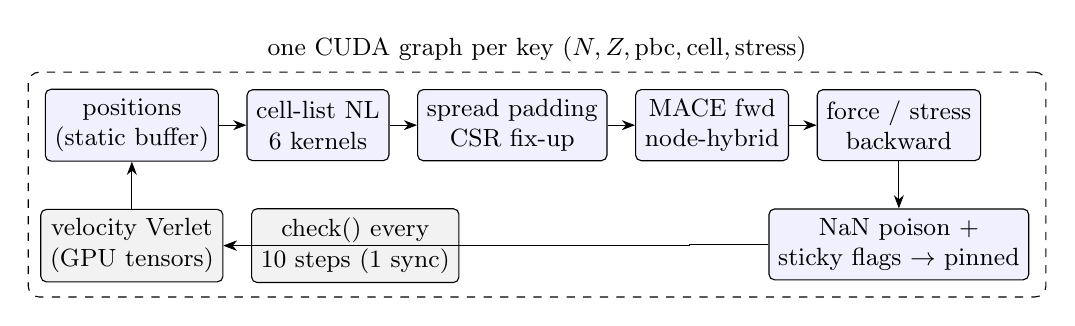
\begin{tikzpicture}[
  box/.style={draw,rounded corners=2pt,minimum height=0.9cm,align=center,font=\small,fill=#1},
  box/.default=white, >=Stealth, node distance=0.35cm]
\node[box=blue!6] (pos) {positions\\(static buffer)};
\node[box=blue!6,right=of pos] (nl) {cell-list NL\\6 kernels};
\node[box=blue!6,right=of nl] (pad) {spread padding\\CSR fix-up};
\node[box=blue!6,right=of pad] (fwd) {MACE fwd\\node-hybrid};
\node[box=blue!6,right=of fwd] (bwd) {force / stress\\backward};
\node[box=blue!6,below=0.6cm of bwd] (flag) {NaN poison +\\sticky flags $\to$ pinned};
\node[draw,dashed,rounded corners,fit=(pos)(nl)(pad)(fwd)(bwd)(flag),inner sep=6pt,label={[font=\small]above:one CUDA graph per key $(N,Z,\text{pbc},\text{cell},\text{stress})$}] (g) {};
\node[box=gray!10,below=0.6cm of pos] (vv) {velocity Verlet\\(GPU tensors)};
\node[box=gray!10,right=of vv] (chk) {check() every\\10 steps (1 sync)};
\draw[->] (pos)--(nl); \draw[->] (nl)--(pad); \draw[->] (pad)--(fwd); \draw[->] (fwd)--(bwd); \draw[->] (bwd)--(flag);
\draw[->] (vv)--(pos); \draw[->] (flag.west) -- ++(-1.0,0) |- (vv.east);
\draw[->,dashed] (chk) -- (vv);
\end{tikzpicture}
\caption{GPU-resident step. One device-to-device copy and one graph launch per force evaluation; the host is consulted once every 10 steps.}
\label{fig:gpustep}
\end{figure}

\subsection{Cell-list neighbour builder}
\code{scripts/nl9/cell\_nl.py} (CUDA via \code{load\_inline}, \code{--fmad=false}) launches six kernels with no host synchronisation and no data-dependent allocation:
\begin{enumerate}
  \item \code{k\_prep}: zero counters; for open systems compute the bounding box with a block reduction, bin widths $\ge r_{\max}(1+10^{-9})$, and MACE's extended cell, reciprocal cell and volume, bitwise equal to the reference.
  \item \code{k\_bin}: one thread per atom; fractional coordinates, wrapping, and \code{atomicAdd} into a fixed-capacity bin. A slot beyond capacity sets overflow bit 2.
  \item \code{k\_wscan<0>}: one \emph{warp per destination atom}. Lanes 0--26 each own one of the 27 neighbour bins and its periodic image; a warp inclusive scan flattens them into one candidate space; lanes stride over candidates, locate their bin by a 5-step binary search, evaluate $d^2$ and count hits with \code{\_\_ballot\_sync}/\code{\_\_popc}.
  \item \code{k\_rowscan2}: a two-level warp-shuffle scan turns per-row counts into \code{rowptr}; the true total $E$ is recorded even when it exceeds $E_{\text{cap}}$ (overflow bit 1).
  \item \code{k\_wscan<1>}: repeats the scan and writes hits. \emph{Sender order without a sort}: within a destination row senders are unique (cell heights $\ge3r_{\max}$ imply one image per pair), so each hit's final slot is its rank among the row's hits, computed deterministically.
  \item \code{k\_final}: one thread per slot. Real edges get unit shifts referred back to the caller's unwrapped positions; the \emph{source CSR permutation} is obtained from the symmetric reverse edge: for edge $(i\to j,S)$ a binary search in row $i$ (sender-sorted) finds the reverse edge $(j\to i,-S)$, whose slot is \code{perm\_src[e]}. A missing reverse edge sets bit 4. Unused slots become padding self-edges.
\end{enumerate}
The output contract is destination-sorted \code{edge\_index}, \code{unit\_shifts}, \code{shifts}, \code{rowptr} (identical for both orders since the list is symmetric), \code{perm\_src}, \code{n\_edges} and a 3-bit \code{overflow} word. The tuple (\code{perm\_dst}, \code{rowptr\_dst}, \code{perm\_src}, \code{rowptr\_src}) is bitwise equal to Phase~8's sort-based \code{build\_csr} in every test.

\paragraph{Bitwise neighbour decisions.} Matching the reference builder edge-for-edge required reproducing floating-point evaluation order. torch evaluates \code{(d*d).sum(-1)} for a length-3 last dimension as $(d_x^2+d_z^2)+d_y^2$, found by probing; the naive order mismatched 945{,}980 of $4\times10^6$ random pairs at the cutoff. Integer-shift products $S\cdot\text{cell}$ must equal cuBLAS's FP64 $[M,3]\times[3,3]$, which we found to be \code{fma(a2,C2, fma(a1,C1, a0*C0))} for all $M$ up to $3\times10^5$; without this, triclinic cells with atoms far outside the box mismatched shifts by $1.4\times10^{-14}$. After both fixes: 0 mismatches. Stock matscipy itself differs from both GPU builders for pairs within $2.7\times10^{-15}$\,\AA{} of $r_{\max}$ (it includes $d=r_{\max}$ exactly); those edges carry envelope weight $\approx0$.

\paragraph{Supported geometries.} Open systems (bounding-box bins, recomputed each build so expanding systems grow bins rather than overflow), and fully periodic orthorhombic or triclinic cells whose perpendicular heights admit $\ge3$ bins of width $\ge r_{\max}$, i.e.\ $\gtrsim15$\,\AA{} at $r_{\max}=5$\,\AA. Atoms may be anywhere, including thousands of \AA{} outside the cell. Smaller cells, mixed periodicity and degenerate cells raise \code{NotImplementedError} and the caller falls back.

\paragraph{Evolution and timing.} A first thread-per-atom version (in-row insertion sort) replayed in 0.17--0.58\,ms; the warp-per-atom rewrite took 0.024--0.085\,ms. \Cref{tab:nltime} compares the final builder with the Phase-5 prototype and matscipy.

\begin{table}[h]
\centering
\caption{Neighbour-list build, median ms (job 1125). ``cell'' is CUDA-graph replay of the new builder; proto includes its host sync.}
\label{tab:nltime}
\small
\begin{tabular}{lrrrrr}
\toprule
System & $N$ & $E$ & cell (replay) & proto (GPU, $O(N^2)$) & matscipy (CPU) \\
\midrule
aspirin & 21 & 302 & 0.024 & 0.432 & 0.091 \\
water192 & 192 & 6{,}634 & 0.034 & 0.452 & 0.893 \\
water648 & 648 & 26{,}550 & 0.042 & 0.479 & 3.996 \\
wbox648 & 648 & 35{,}698 & 0.052 & 1.460 & 8.115 \\
wclus2187 & 2{,}187 & 99{,}438 & 0.050 & 0.698 & 14.594 \\
wbox2187 & 2{,}187 & 120{,}506 & 0.060 & 8.036 & 21.547 \\
wclus5184 & 5{,}184 & 247{,}652 & 0.075 & 1.712 & 42.883 \\
wbox5184 & 5{,}184 & 285{,}464 & 0.081 & 42.916 & 57.837 \\
\bottomrule
\end{tabular}
\end{table}

\subsection{The captured step (GPUStep)}
\code{scripts/int9/gpu\_step.py} captures, per key, the builder, a padding fix-up, the model forward and force (and optionally stress) backward, an overflow guard, and an asynchronous copy of device flags to pinned host memory. A call is one device-to-device copy into the static position buffer plus \code{graph.replay()}: zero host synchronisations. The convolution receives the builder's CSR through an external holder (\code{nodeconv\_ext.py}) identified by object identity, so no sort runs inside the model; the only remaining sorts in the step are MACE's own \code{index} backward, present in every backend.

\paragraph{Padding must be spread.} The builder places all $P=E_{\text{cap}}-E$ padding edges on node $N-1$, which keeps both orders sorted. Inside the model this was catastrophic: one CTA of the node-centric convolution received $\sim$$P$ edges, and MACE's index backward accumulated $P$ duplicates into one row. Steps became 10--40$\times$ slower (water2187: 126\,ms vs 9.3\,ms; wbox5184: 1{,}969\,ms vs 24\,ms). The fix re-homes padding edge $k$ to node $k\bmod N$ and rebuilds both CSRs without a sort in $O(E_{\text{cap}})$ elementwise work: with $c_n=\#\{k<P:k\bmod N=n\}=\max(0,\lfloor(P-n+N-1)/N\rfloor)$ and its exclusive prefix sum $\bar c_n$, real edge $e$ with destination $d$ moves to slot $e+\bar c_d$, padding $k$ to $\text{rowptr}'_n+\deg_n+\lfloor k/N\rfloor$, and likewise for the source order. This costs $\sim$50\us{} and is the main reason \Bone{} is slightly slower than Phase~8's.

\paragraph{Overflow can never look valid.} If any overflow bit is set, the real-edge count and row pointers are forced to zero so the model sees a \emph{consistent all-padding graph} (an earlier version fed an inconsistent CSR and triggered an illegal memory access that destroyed the CUDA context), and energy, forces and stress are poisoned with NaN. Flags are sticky. \code{check()} performs one counted synchronisation, reads the flags, and recaptures with $E_{\text{cap}}=\lceil1.25E_{\max}\rceil_{64}$ (or a larger bin capacity) on overflow, returning \code{ok=False} so the caller rolls back; it also recaptures proactively when $E_{\max}>0.98E_{\text{cap}}$. A caller that never checks receives NaN, never a plausible wrong number.

\paragraph{Capture hygiene.} Python's cyclic garbage collector, freeing an old graph's pinned buffer during a new capture, caused the caching host allocator to record a CUDA event inside the capture and invalidate it. GC is now disabled across warm-up and capture.

\paragraph{Fallbacks.} Unsupported geometries use Phase~8's runner with the prototype builder (synchronising, outside the graph). A capturable $O(N^2)$ brute-force builder exists but materialises $[B,27,N,3]$ candidate tensors, compacts with a cumulative sum and three scatters over all candidates (all non-hits written to one dump slot), then sorts; at wbox192 it took $\sim$4.3\,ms, slower than the synchronising fallback (2.38\,ms), so it is not used automatically.

\subsection{GPU velocity Verlet}
\code{scripts/md9/vv.py} implements ASE's momentum-form velocity Verlet on FP64 GPU tensors. Potential and kinetic energy are written to preallocated device buffers at a device-side step index, so logging needs no synchronisation. Every 10 steps the integrator calls \code{check()}; on success it checkpoints $(x,p,F)$ by device copies, on overflow it rolls back and repeats. Over all Phase-9 MD runs there were zero overflows, rollbacks or recaptures. A version that also captures the two half-kicks as small graphs (\code{gpustep\_cg}) gained at most 0.6\%.

\subsection{Correctness}
\begin{table}[h]
\centering
\caption{Phase 9 correctness, all passing (tolerances $10^{-11}$\,eV/atom, $10^{-11}$\,\eVA, $10^{-14}$\,eV/\AA$^3$).}
\label{tab:corr9}
\small
\begin{tabular}{p{6.4cm}rrrr}
\toprule
Test & samples & $|\Delta E|/N$ & $\max|\Delta F|$ & $|\Delta\sigma|$ \\
\midrule
Builder: edge sets, CSR, boundary pairs at $r_{\max}\pm$ulp, overflow, capture; 17 systems (job 1122) & 187 & --- & --- & --- \\
Builder batch through stock model & --- & 9.0e-13 & 8.5e-14 & $\le$9.7e-17 \\
GPUStep vs stock, 10 systems, 7-config walks, stress (job 1144) & 98 & 1.1e-12 & 2.1e-14 & 7.0e-17 \\
GPUStep vs Phase-8 node-hybrid + proto & 98 & 6.3e-13 & \textbf{0 (bitwise)} & 1.3e-17 \\
Overflow, proactive recapture, compression walk, bin overflow & 20 & 1.5e-13 & 3.6e-13 & 0 \\
Species-order and atom-count traps & 7 & 1.7e-13 & 8.5e-13 & 0 \\
Fallback paths (wbox192, mixed pbc) & 15 & 1.5e-13 & 7.1e-15 & 5.6e-17 \\
Zero-edge and tiny systems & 3 & 0 & 1.0e-15 & 0 \\
MD: 10 systems $\times$ 3 providers, 500--1000 steps, sampled on identical coordinates & 51--201 each & 1.3e-12 & 8.4e-15 & 4.7e-17 \\
Negative control: one edge dropped & 5/5 fail & 8.8e-4 & 0.42 & --- \\
\bottomrule
\end{tabular}
\end{table}

At every sampled MD step the neighbour set matched stock bitwise; an isolated atom always had exactly zero force; GPUStep and the Phase-8 graphed path produced \emph{bitwise-identical trajectories} over 2\,ps, meaning the builder reproduces the Phase-8 stable-sort edge order exactly. NVE drift matched stock within block noise (\cref{tab:drift9}). One excluded case: with atoms $\sim$3{,}000\,\AA{} outside the cell, stress differed from stock by $1.1\times10^{-14}$ in one run, the same size as the reference builder's own noise there (atomics $\times$ large coordinates); it passes at $8.2\times10^{-15}$ in the final run and the global tolerance was not loosened.

\begin{table}[h]
\centering
\caption{NVE drift over 2\,ps, eV/atom/ps $\pm$ std of 4 block slopes.}
\label{tab:drift9}
\small
\begin{tabular}{lrrr}
\toprule
System, $\Delta t$ & stock eager & Phase-8 graphed & GPUStep \\
\midrule
water192, 0.5\,fs & $-5.78\times10^{-6}\pm1.8\times10^{-6}$ & $-5.95\times10^{-6}\pm1.9\times10^{-6}$ & $-5.95\times10^{-6}\pm1.9\times10^{-6}$ \\
wbox648, 0.5\,fs & $-8.54\times10^{-6}\pm4.2\times10^{-6}$ & $-1.16\times10^{-5}\pm4.7\times10^{-6}$ & $-1.16\times10^{-5}\pm4.7\times10^{-6}$ \\
wbox648, 0.25\,fs & $-2.53\times10^{-6}\pm1.2\times10^{-6}$ & $-2.86\times10^{-6}\pm1.1\times10^{-6}$ & $-2.86\times10^{-6}\pm1.1\times10^{-6}$ \\
\bottomrule
\end{tabular}
\end{table}

\section{End-to-end results and attribution}
\label{sec:results}

\subsection{The ladder}
\Cref{fig:ladder} follows two systems through the phases at a constant \emph{model-only} boundary (prebuilt graph on GPU, forward+force backward), which is the only boundary measured in every phase. \Cref{tab:ladder} gives the same numbers.

\begin{figure}[h]
\centering
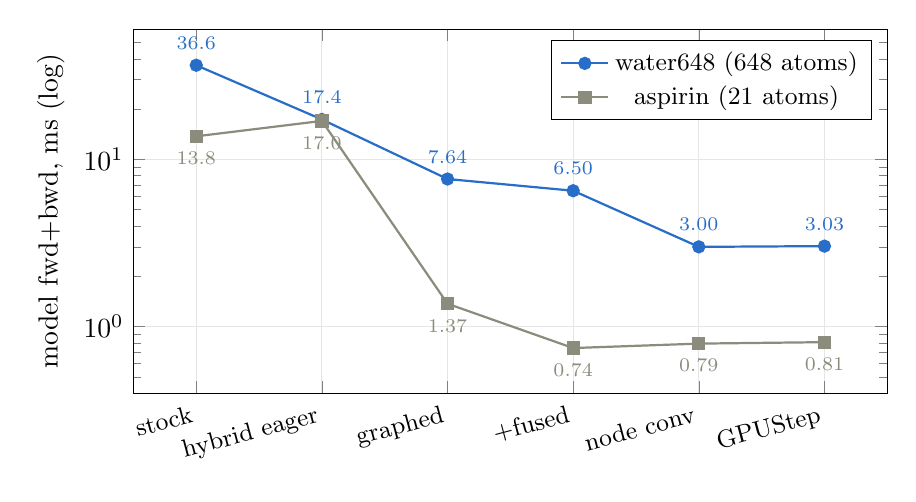
\begin{tikzpicture}
\begin{axis}[
  width=0.92\textwidth, height=6.2cm,
  ymode=log, log basis y=10,
  ylabel={model fwd+bwd, ms (log)},
  symbolic x coords={stock,hybrid eager,graphed,+fused,node conv,GPUStep},
  xtick=data, x tick label style={font=\small,rotate=15,anchor=north east},
  ymin=0.4, ymax=60,
  legend style={at={(0.98,0.97)},anchor=north east,font=\small},
  grid=major, grid style={gray!20},
  nodes near coords, every node near coord/.append style={font=\scriptsize},
  point meta=explicit symbolic]
\addplot[mark=*,thick,cnew,every node near coord/.append style={anchor=south,yshift=2pt}] coordinates {
  (stock,36.63)[36.6] (hybrid eager,17.35)[17.4] (graphed,7.64)[7.64] (+fused,6.50)[6.50] (node conv,3.00)[3.00] (GPUStep,3.03)[3.03]};
\addplot[mark=square*,thick,cnode,every node near coord/.append style={anchor=north,yshift=-2pt}] coordinates {
  (stock,13.76)[13.8] (hybrid eager,17.01)[17.0] (graphed,1.37)[1.37] (+fused,0.744)[0.74] (node conv,0.791)[0.79] (GPUStep,0.807)[0.81]};
\legend{water648 (648 atoms), aspirin (21 atoms)}
\end{axis}
\end{tikzpicture}
\caption{Model-only time (prebuilt graph) through the phases. GPUStep's value includes its in-graph neighbour build. Sources: profile6 (stock, hybrid eager), validate7 PROFILE (graphed), validate7 (fused), prof8 (node), int9 final (GPUStep \Bone).}
\label{fig:ladder}
\end{figure}

\begin{table}[h]
\centering
\caption{Phase attribution at the model-only boundary, ms; factor relative to the previous step.}
\label{tab:ladder}
\small
\begin{tabular}{lrrrr}
\toprule
Step & water648 & factor & aspirin & factor \\
\midrule
Stock e3nn, eager (Phase 6) & 36.63 & --- & 13.76 & --- \\
Hybrid (FlashTP FP64-CG + cueq SC), eager & 17.35 & 2.11$\times$ & 17.01 & \textcolor{cbad}{0.81$\times$} \\
Hybrid, CUDA graph & 7.64 & 2.27$\times$ & 1.37 & 12.4$\times$ \\
+ fused embedding + fused node op & 6.50 & 1.18$\times$ & 0.744 & 1.84$\times$ \\
Node-centric convolution (node-hybrid) & 3.00 & 2.17$\times$ & 0.791 & \textcolor{cbad}{0.94$\times$} \\
GPUStep \Bone{} (includes neighbour build) & 3.03 & 0.99$\times$ & 0.807 & 0.98$\times$ \\
\midrule
\textbf{Total} & & \textbf{12.1$\times$} & & \textbf{17.1$\times$} \\
\bottomrule
\end{tabular}
\end{table}

The phases did very different work at the two sizes: at aspirin, CUDA graphs and the reduction of graph nodes by fusion account for almost all of the gain; at 648 atoms the gain is spread over kernel replacement (2.1$\times$), capture (2.3$\times$) and the node-centric convolution (2.2$\times$). Two steps lost time at aspirin (the eager hybrid and the node convolution), which we kept because they won at the sizes that matter for MD.

\subsection{Final apples-to-apples timing}
\Cref{tab:final} is the Phase-9 comparison of all four backends at all three boundaries on the same GPUs, runs A (job 1145) and B (job 1146) agreeing within 2\%; \Bthree{} is from job 1147 (stock \Bthree{} uses ASE, jobs 1084/1129). \Cref{fig:final-speedup} plots the \Btwo{} speedups.

\begin{table}[p]
\centering
\caption{Final timings, median ms (run A). \Bone: replay with prebuilt graph (GPUStep includes its NL). \Btwo: complete step from GPU-resident coordinates. \Bthree: sustained MD ms/step. FlashTP-hyb = Phase-7 graphed hybrid+fused; node-hyb = Phase 8.}
\label{tab:final}
\small
\begin{tabular}{llrrrrr}
\toprule
System & Backend & \Bone & \Btwo & \Bthree & \Btwo{} vs stock & peak MiB \\
\midrule
\multirow{4}{*}{aspirin (21)} & stock & 11.61 & 16.34 & --- & 1.0 & 113 \\
 & FlashTP-hyb & 0.679 & 0.910 & --- & 18.0 & 143 \\
 & node-hyb & 0.754 & 0.938 & 1.366 & 17.4 & 77 \\
 & \textbf{GPUStep} & 0.807 & \textbf{0.814} & \textbf{0.896} & \textbf{20.1} & 77 \\
\midrule
\multirow{4}{*}{water192} & stock & 13.45 & 18.10 & 18.03 & 1.0 & 1132 \\
 & FlashTP-hyb & 2.188 & 2.372 & --- & 7.6 & 312 \\
 & node-hyb & 1.517 & 1.704 & 2.133 & 10.6 & 296 \\
 & \textbf{GPUStep} & 1.553 & \textbf{1.560} & \textbf{1.601} & \textbf{11.6} & 296 \\
\midrule
\multirow{4}{*}{wbox192 (P)} & stock & 15.82 & 22.01 & --- & 1.0 & 1623 \\
 & FlashTP-hyb & 2.948 & 3.605 & --- & 6.1 & 443 \\
 & node-hyb & 1.730 & 2.380 & 2.784 & 9.2 & 423 \\
 & GPUStep (fallback) & 1.739 & 2.414 & 2.342 & 9.1 & 423 \\
\midrule
\multirow{4}{*}{org648} & stock & 27.87 & 35.21 & --- & 1.0 & 2857 \\
 & FlashTP-hyb & 4.185 & 4.374 & --- & 8.0 & 642 \\
 & node-hyb & 2.320 & 2.514 & 2.980 & 14.0 & 598 \\
 & \textbf{GPUStep} & 2.352 & \textbf{2.360} & \textbf{2.409} & \textbf{14.9} & 597 \\
\midrule
\multirow{4}{*}{water648} & stock & 36.39 & 45.45 & 45.86 & 1.0 & 4307 \\
 & FlashTP-hyb & 6.481 & 6.682 & --- & 6.8 & 1039 \\
 & node-hyb & 2.989 & 3.183 & 3.643 & 14.3 & 981 \\
 & \textbf{GPUStep} & 3.028 & \textbf{3.044} & \textbf{3.082} & \textbf{14.9} & 976 \\
\midrule
\multirow{4}{*}{wbox648 (P)} & stock & 43.21 & 56.29 & 55.96 & 1.0 & 5445 \\
 & FlashTP-hyb & 8.382 & 9.584 & --- & 5.9 & 1339 \\
 & node-hyb & 3.667 & 4.851 & 5.236 & 11.6 & 1270 \\
 & \textbf{GPUStep} & 3.723 & \textbf{3.733} & \textbf{3.773} & \textbf{15.1} & 1265 \\
\midrule
\multirow{4}{*}{water2187} & stock & 120.9 & 141.8 & 143.9 & 1.0 & 15720 \\
 & FlashTP-hyb & 22.66 & 23.06 & --- & 6.1 & 3653 \\
 & node-hyb & 9.181 & 9.568 & 10.148 & 14.8 & 3450 \\
 & \textbf{GPUStep} & 9.248 & \textbf{9.251} & \textbf{9.310} & \textbf{15.3} & 3440 \\
\midrule
\multirow{4}{*}{wbox2187 (P)} & stock & 136.4 & 208.7 & 210.1 & 1.0 & 18332 \\
 & FlashTP-hyb & 26.83 & 34.52 & --- & 6.0 & 4295 \\
 & node-hyb & 10.66 & 18.36 & 18.88 & 11.4 & 4130 \\
 & \textbf{GPUStep} & 10.74 & \textbf{10.74} & \textbf{10.84} & \textbf{19.4} & 4111 \\
\midrule
\multirow{4}{*}{water5184} & stock & 290.5 & 400.5 & 397.6 & 1.0 & 38714 \\
 & FlashTP-hyb & 55.48 & 56.81 & --- & 7.0 & 8905 \\
 & node-hyb & 21.22 & 22.53 & 23.27 & 17.8 & 8408 \\
 & \textbf{GPUStep} & 21.35 & \textbf{21.37} & \textbf{21.54} & \textbf{18.7} & 8382 \\
\midrule
\multirow{4}{*}{wbox5184 (P)} & stock & 319.3 & 445.6 & 437.8 & 1.0 & 43406 \\
 & FlashTP-hyb & 63.26 & 105.57 & --- & 4.2 & 10169 \\
 & node-hyb & 23.78 & 66.05 & 66.84 & 6.7 & 9628 \\
 & \textbf{GPUStep} & 23.90 & \textbf{23.95} & \textbf{24.09} & \textbf{18.6} & 9575 \\
\bottomrule
\end{tabular}
\end{table}

\begin{figure}[h]
\centering
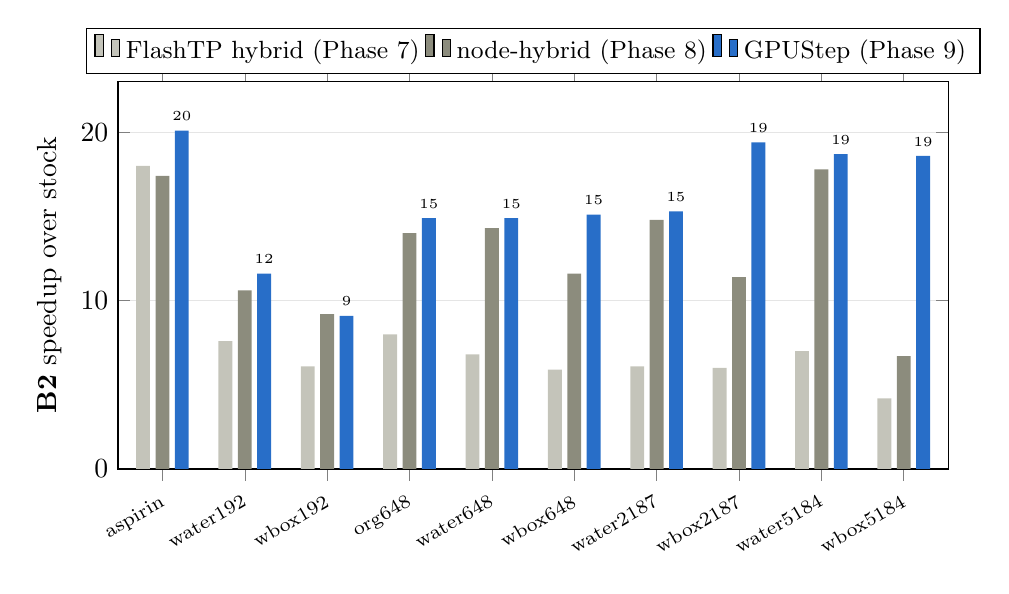
\begin{tikzpicture}
\begin{axis}[
  ybar, bar width=5pt,
  width=\textwidth, height=6.5cm,
  ylabel={\Btwo{} speedup over stock},
  symbolic x coords={aspirin,water192,wbox192,org648,water648,wbox648,water2187,wbox2187,water5184,wbox5184},
  xtick=data, x tick label style={font=\scriptsize,rotate=30,anchor=north east},
  ymin=0, ymax=23, enlarge x limits=0.06,
  legend style={at={(0.5,1.02)},anchor=south,legend columns=3,font=\small},
  grid=major, grid style={gray!20}, ymajorgrids=true, xmajorgrids=false]
\addplot[fill=cflash,draw=none] coordinates {(aspirin,18.0)(water192,7.6)(wbox192,6.1)(org648,8.0)(water648,6.8)(wbox648,5.9)(water2187,6.1)(wbox2187,6.0)(water5184,7.0)(wbox5184,4.2)};
\addplot[fill=cnode,draw=none] coordinates {(aspirin,17.4)(water192,10.6)(wbox192,9.2)(org648,14.0)(water648,14.3)(wbox648,11.6)(water2187,14.8)(wbox2187,11.4)(water5184,17.8)(wbox5184,6.7)};
\addplot[fill=cnew,draw=none,nodes near coords,every node near coord/.append style={font=\tiny,/pgf/number format/fixed,/pgf/number format/precision=0}] coordinates {(aspirin,20.1)(water192,11.6)(wbox192,9.1)(org648,14.9)(water648,14.9)(wbox648,15.1)(water2187,15.3)(wbox2187,19.4)(water5184,18.7)(wbox5184,18.6)};
\legend{FlashTP hybrid (Phase 7), node-hybrid (Phase 8), GPUStep (Phase 9)}
\end{axis}
\end{tikzpicture}
\caption{Complete-step (\Btwo) speedup over stock eager FP64 MACE. wbox = periodic; wbox192 uses the fallback builder.}
\label{fig:final-speedup}
\end{figure}

\paragraph{Reading the table.}
\begin{itemize}
  \item GPUStep's \Bone{} is 0.04--0.2\,ms \emph{above} node-hybrid's at $\ge$2{,}187 atoms (it includes the 0.05--0.08\,ms builder and the $\sim$50\us{} padding fix-up), but its \Btwo{} is the best everywhere it applies, because it is equal to its \Bone{}.
  \item Phase~9 gains 1.71$\times$ (wbox2187) and 2.76$\times$ (wbox5184) over Phase~8 at \Btwo{} for periodic boxes, and only 1.03--1.09$\times$ for clusters, where the old builder was 3--6\% of the step.
  \item \Bthree{} tracks \Btwo{} within 0.02--0.18\,ms: integration and the every-10-steps check are nearly free. Against stock ASE MD, sustained throughput is 11.4$\times$ (water192) to 19.4$\times$ (wbox2187).
  \item The same graph with the FlashTP convolution instead of the node convolution (``GPUStep w/ FlashTP'', not shown) was never faster (aspirin 0.872 vs 0.814\,ms), so no small-$N$ dispatch is needed.
  \item Peak memory is unchanged from node-hybrid and 4.5$\times$ below stock at 5{,}184 atoms (9.6 vs 43.4\,GB); by memory, node-hybrid would fit $\sim$40{,}000 water atoms on 80\,GB versus $\sim$9{,}000 for stock.
  \item Host synchronisations per MD step: stock 38, ASE 43, Phase-8 graphed 2 (clusters) to 30 (wbox5184), GPUStep 0 (+0.1 from \code{check()}).
  \item First capture costs 0.24--0.84\,s per key; build/install 0.47\,s.
\end{itemize}

\subsection{Where the remaining time goes}
\begin{figure}[h]
\centering
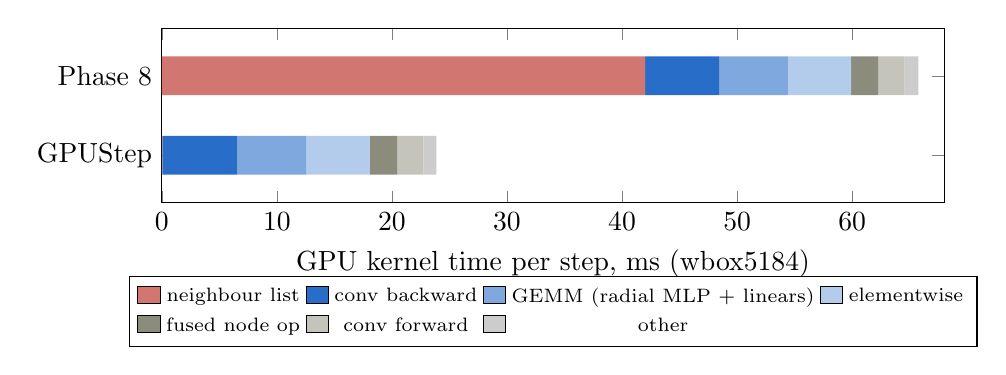
\begin{tikzpicture}
\begin{axis}[
  xbar stacked, bar width=14pt,
  width=0.95\textwidth, height=3.8cm, enlarge y limits=0.6,
  xlabel={GPU kernel time per step, ms (wbox5184)},
  symbolic y coords={GPUStep,Phase 8},
  ytick=data, xmin=0, xmax=68,
  legend style={at={(0.5,-0.42)},anchor=north,legend columns=4,font=\scriptsize},
  reverse legend=false]
\addplot[fill=cbad!70,draw=none] coordinates {(41.995,Phase 8) (0.052,GPUStep)};
\addplot[fill=cnew,draw=none] coordinates {(6.441,Phase 8) (6.518,GPUStep)};
\addplot[fill=cnew!60,draw=none] coordinates {(5.981,Phase 8) (5.975,GPUStep)};
\addplot[fill=cnew!35,draw=none] coordinates {(5.483,Phase 8) (5.546,GPUStep)};
\addplot[fill=cnode,draw=none] coordinates {(2.370,Phase 8) (2.367,GPUStep)};
\addplot[fill=cflash,draw=none] coordinates {(2.294,Phase 8) (2.269,GPUStep)};
\addplot[fill=gray!40,draw=none] coordinates {(1.196,Phase 8) (1.137,GPUStep)};
\legend{neighbour list, conv backward, GEMM (radial MLP + linears), elementwise, fused node op, conv forward, other}
\end{axis}
\end{tikzpicture}
\caption{Profile of one step at wbox5184 (job 1145, torch.profiler). The neighbour list falls from 42.0\,ms to 0.05\,ms; the model is unchanged.}
\label{fig:profile}
\end{figure}

\begin{table}[h]
\centering
\caption{GPU kernel time per step, \us{} (share), GPUStep (job 1145).}
\label{tab:prof9}
\small
\begin{tabular}{lrrr}
\toprule
Category & wbox5184 & water5184 & wbox2187 \\
\midrule
conv backward (node) & 6518 (27.3\%) & 5651 (26.5\%) & 2901 (27.1\%) \\
GEMM (radial MLP + linears) & 5975 (25.0\%) & 5229 (24.5\%) & 2639 (24.7\%) \\
elementwise & 5546 (23.2\%) & 4928 (23.1\%) & 2484 (23.2\%) \\
fused node op & 2367 (9.9\%) & 2365 (11.1\%) & 1022 (9.6\%) \\
conv forward (node) & 2269 (9.5\%) & 2020 (9.5\%) & 1005 (9.4\%) \\
cueq symmetric contraction & 487 (2.0\%) & 486 (2.3\%) & 215 \\
scatter/gather/index & 261 & 237 & 167 \\
fused embedding & 232 & 202 & 106 \\
sort/search (MACE index bwd) & 85 & 83 & 55 \\
neighbour list & 52 & 49 & 40 \\
\midrule
kernel sum / wall & 23{,}864 / 23{,}976 & 21{,}320 / 21{,}416 & 10{,}685 / 10{,}778 \\
\bottomrule
\end{tabular}
\end{table}

The step is now $\sim$99\% GPU-busy and 100\% model (\cref{fig:profile,tab:prof9}). The top individual kernels at wbox5184 are the node backward (6.5\,ms), an \code{AUnaryFunctor<double>} elementwise kernel (2.9\,ms), an \code{sm90} FP64 GEMM (2.7\,ms), the fused node GEMM (2.4\,ms), SiLU (1.8\,ms) and the node forward (1.6\,ms). At aspirin, by contrast, the GPU is busy only 756 of 1{,}247\us{} under the profiler: small systems remain launch-latency-bound even inside a graph.

\clearpage
\section{Negative results, bugs and dead ends}
\label{sec:negative}

We list everything that failed, regressed, or was abandoned, with its measured cost, because several of these are traps that the next person optimising an equivariant MLIP will meet.

\small
\begin{longtable}{p{0.5cm}p{4.4cm}p{6.0cm}p{4.0cm}}
\caption{Ledger of negative results.}\label{tab:negative}\\
\toprule
\# & What & Evidence & Outcome \\
\midrule
\endfirsthead
\toprule
\# & What & Evidence & Outcome \\
\midrule
\endhead
\multicolumn{4}{l}{\emph{Correctness traps}}\\
1 & FlashTP FP64 rounds CG to FP32 & $3$--$10\times10^{-8}$\,\eVA; upstream test passes & Patched (\cref{sec:precision}) \\
2 & FlashTP CG precision follows global default dtype & first fix silently FP32 under default float32 & Second patch \\
3 & FlashTP \code{extcg} kernel keeps a \code{float} path norm & caps NequIP-style configs at $2.5\times10^{-8}$ & Documented, not fixed (needs rebuild) \\
4 & FlashTP crashes at $E=0$ & ``invalid configuration argument'' & Adapter bypass \\
5 & Edge-index cache keyed on \code{data\_ptr} & allocator reuse $\Rightarrow$ 13--79\,\eVA{} errors on walks & Cache removed \\
6 & Stock FlashTP not captured by CUDA graph & capture ``succeeds''; 576\,\eVA{} error & Stream patch; parity-gated capture \\
7 & Graph reuse across species order & reversed aspirin: 6.7\,eV/atom, 308\,\eVA{} & Keyed graphs \\
8 & Graph reuse across $N$ & stale padding index & Keyed graphs \\
9 & NL distance sum order & 945{,}980/4M boundary mismatches & Match torch order \\
10 & NL shift product order & triclinic far-outside shifts off by $1.4\times10^{-14}$ & Match cuBLAS FMA order \\
11 & Bin overflow with inconsistent CSR & illegal memory access, lost context & All-padding graph + NaN \\
12 & GC during capture & capture invalidated (abort) & GC disabled around capture \\
13 & \code{empty}-allocated gradients for uncovered edges & garbage $\partial y,\partial w$ if CSR misses padding & CSR must cover all $E_{\text{cap}}$ \\
\midrule
\multicolumn{4}{l}{\emph{Performance regressions and rejected ideas}}\\
14 & cuEquivariance eagerly at small $N$ & 0.52--0.76$\times$ stock (10\,ms host floor); 10.8\,s first call & Use only its SC, only under graphs \\
15 & Hybrid eagerly below $\sim$400 atoms & 0.79--0.88$\times$ stock & Fixed by CUDA graphs \\
16 & Graphed e3nn (padding, no kernel change) & slower than eager at 648 (38.3 vs 36.7\,ms) & Abandoned \\
17 & Megakernel & $\le$0.1--0.3\,ms attainable & Not built (\cref{sec:cudagraph}) \\
18 & Triton L1 \code{skip\_tp} at aspirin & +13\us{} vs stock & Kept (net win elsewhere) \\
19 & LunaTP-style path grouping in our forward & slower (re-gathers $x$, register pressure) & Disabled \\
20 & $G=8$ edge slices & register spills & Capped at $G\le4$ \\
21 & Node conv at H$_2$O/aspirin & 0.89/0.95$\times$ (CSR sort, 21 CTAs) & Partly fixed in Phase 9 \\
22 & All padding on last node & 10--40$\times$ slower steps (wbox5184: 1{,}969\,ms) & Spread padding \\
23 & Thread-per-atom cell list & 0.17--0.58\,ms & Warp-per-atom (0.02--0.08\,ms) \\
24 & Capturable $O(N^2)$ small-cell builder & $\sim$4.3\,ms at wbox192 vs 2.38\,ms fallback & Not used automatically \\
25 & Separate small graphs for VV half-kicks & $\le$0.6\% gain & Optional \\
26 & Many graphs in one process & OOM, 29\,GB in graph pools & One process per large system \\
\midrule
\multicolumn{4}{l}{\emph{Measurement and process issues}}\\
27 & Phase-6 eager baselines $\sim$10\% slow & speedups inflated 7--10\% & Corrected by independent validation \\
28 & ``graph pool MiB'' column mislabelled & was peak during capture & Relabelled \\
29 & Phase-1 JSONs overwritten & numbers survive in logs, within 2\% & Noted \\
30 & Three different ``wbox648'' files & 35{,}724 / 35{,}698 / 35{,}198 edges & Never compared across \\
31 & Transient 5--16$\times$ slow jobs (05:31--05:48) & drift runs only & Reran; bitwise identical energies \\
32 & Script overwritten while bash read it & spurious exit 127 & Runs verified exit 0 \\
33 & Patch notes diffstat & said $+43/-6$ for one file; actual $+37/-6$ & Corrected in review \\
\bottomrule
\end{longtable}

\subsection{Lessons}
\begin{enumerate}
  \item \textbf{Re-score library tests at your own tolerance.} FlashTP's FP64 harness tests FP32-grade agreement. ``All Good'' meant nothing for an FP64 claim.
  \item \textbf{A capture that raises nothing may contain nothing.} Every graph must be checked against eager output, not against the absence of an exception.
  \item \textbf{A graph is a function of more than shapes.} Species order, $N$, cell and every captured static are part of the key.
  \item \textbf{Padding placement is a performance parameter.} ``Put the padding at the end'' is correct for sorting and disastrous for a destination-owned kernel.
  \item \textbf{Bitwise equality with a reference requires matching evaluation order}, including the reduction order of a three-element sum and cuBLAS's FMA chain.
  \item \textbf{Overflow handling must produce a consistent but obviously wrong result}, never a plausible one and never undefined memory.
  \item \textbf{Measure the next bottleneck before building.} Each phase's profile predicted the next phase's gain within $\sim$30\%, and twice prevented building something unnecessary (the megakernel; a small-$N$ FlashTP dispatch).
\end{enumerate}

\section{Discussion}
\label{sec:discussion}

\subsection{What is and is not new}
Almost every component has prior art (\cref{tab:provenance}). The node-centric organisation is LunaTP's; fused tensor-product convolutions beating cuEquivariance are reported by FlashTP, OpenEquivariance, LunaTP and e3j; padded edge buffers with recapture on overflow are what e3j and MACE's own \code{compile\_mode} do; GPU cell lists with overflow flags are standard in classical MD. What appears new is narrower: a fully capturable FP64 MACE-OFF step in which the neighbour builder emits the convolution's CSR directly; a single fused atomic-free source-centric backward; the FlashTP FP64 CG finding; and a careful demonstration that all of this composes without moving the FP64 result by more than $\sim10^{-12}$. A defensible one-line claim is ``the fastest measured FP64 MACE-OFF23-medium single-system complete step on H100 \emph{among the backends we measured}, at accuracy indistinguishable from stock''.

\subsection{Missing baselines}
The 12--20$\times$ headline is measured against \emph{eager e3nn}, which is how MACE runs by default but not its fastest configuration. Three comparisons are needed before any state-of-the-art claim:
\begin{enumerate}
  \item \textbf{MACE + cuEquivariance + \code{torch.compile(mode="reduce-overhead")}}. This attacks the same launch floor as our CUDA graphs, and the installed MACE~0.3.17 supports it (\code{compile\_mode=}). We expect it to close most of the gap at small $N$; against it, our margin will be substantially smaller than 12--20$\times$, and that smaller number is the one that matters.
  \item \textbf{MACE's cueq-SC + OpenEquivariance-conv hybrid} (v0.3.16+) under the same compile mode, at \Btwo.
  \item \textbf{LunaTP inside a captured step}, which would require making its \code{make\_graph} capturable; our bound suggests 1.08--1.21$\times$ further at the whole-model level.
\end{enumerate}
External numbers are not directly comparable: e3j's 4.9\,ms/step for 1{,}503 atoms is FP32, NPT, and a correlation-2 custom MACE; OpenEquivariance's 6.2$\times$ FP64 figure is against unoptimised MACE on an unstated GPU. Our FP64 3.7\,ms at 648 periodic atoms and 10.7\,ms at 2{,}187 are in the same range, which is encouraging but proves nothing either way.

\subsection{Was the $10^{-11}$ gate the right design constraint?}
It was an excellent regression test: it caught the FlashTP CG bug, an edge-cache bug, two capture hazards and a padding bug that a physical tolerance would have missed or only caught late. As a \emph{design constraint}, however, it ruled out the largest remaining lever, precision. The model's own force error versus DFT is $\sim$10\,meV/\AA, eight orders of magnitude above the gate, and most production MLIP MD does not run in FP64. The remaining profile is half FP64 GEMMs and FP64 convolution backward. A mixed-precision path (radial MLP in FP32/TF32, FP64 accumulation in the convolution) should be evaluated against a separate \emph{physical} gate: force error relative to the model-vs-DFT error distribution, NVE drift, and structural observables. The FP64 path and its tight gate should stay as the reference.

\subsection{Concrete next steps}
\paragraph{Fold the radial MLP's last layer into the convolution.} The radial MLP ends in a bias-free linear layer, so $w_e = h_e A$ with $h_e\in\mathbb R^{64}$ the last hidden activation and $A\in\mathbb R^{64\times1280}$ (L1). The convolution could read $h_e$ (512\,B/edge) and hold $A$ in shared memory instead of reading $w_e$ (10\,KB/edge), cutting the dominant memory stream $\sim$20$\times$ and absorbing part of the 25\% GEMM share. This is the idea behind Sobek's streaming formulation~\cite{sobek}, which treats a linear radial projection and has only been benchmarked in FP32 on synthetic graphs; an FP64 MACE implementation would be new. The backward needs $\partial h_e = \partial w_e A^\top$, which can be fused into the source-centric kernel.
\paragraph{Split the backward for occupancy.} The node backward is 27\% and runs one CTA per source node at 238-register pressure; splitting by channel chunk or path group at small $N$ and moving $y$ to shared memory are the obvious next experiments.
\paragraph{Fix the small-cell builder.} At 192 atoms with 27 images there are $\sim10^6$ candidate pairs, which a single fused kernel should evaluate in tens of microseconds. The 4.3\,ms of the existing stub is almost certainly implementation (dense $[B,27,N,3]$ temporaries, three scatters with all misses contending on one dump slot, a full sort), not an inherent limit of brute force. Fixing it removes the only geometry where Phase~9 did not improve.
\paragraph{Avoid recapture for NPT.} CUDA graphs capture pointers, not values. If the cell matrix lives in a fixed device tensor and the bin grid is sized for the largest expected box (with empty bins tolerated), a cell update in place should not require recapture; only a change in grid dimensions would. This needs the builder's periodic geometry, currently fixed at construction, to be read from device memory each build.
\paragraph{Emit spread padding from the builder} to recover the $\sim$50\us{} \Bone{} regression.
\paragraph{Measure throughput, not only latency.} Everything here is single-system latency. For screening many small molecules (aspirin-sized ligands, conformers), batching $B$ systems into one graph removes the launch floor without CUDA-graph machinery and may change which convolution wins; whether the node-centric kernel still leads at, say, $64\times21$ atoms is unmeasured.

\subsection{Threats to validity}
All results are from one GPU model, one node and one model size (MACE-OFF23 medium); MACE-OFF23 large ($L_{\max}=2$, 192 channels) changes register pressure and may change kernel rankings. The systems are water and organic clusters; dense inorganic materials with higher coordination were not tested. Stock timings at $\ge$2{,}187 atoms use 10 repetitions and show larger spreads (e.g.\ wbox5184 \Btwo{} p10--p90 387--471\,ms). The study was executed largely by software agents under a human-written brief; every number in this report was re-read from result files, but the provenance of individual design choices is recorded in agent reports rather than lab notebooks.

\section{Conclusion}
\label{sec:conclusion}

Starting from stock MACE-OFF23 medium in FP64, nine measured steps brought a complete energy+force evaluation on one H100 to 0.81\,ms at 21 atoms, 3.0\,ms at 648 atoms and 23.9\,ms at 5{,}184 atoms in a periodic box (12--20$\times$ at the complete-step boundary), with zero host synchronisations per MD step, forces within $2\times10^{-14}$\,\eVA{} of stock, and NVE drift indistinguishable from stock. The largest single factors were CUDA-graph capture for small systems (12$\times$ at aspirin), and the node-centric convolution plus GPU cell list for large ones (2.2$\times$ and 2.8$\times$). At $\ge$2{,}000 atoms the step is now $\sim$99\% GPU-busy inside the model, so further progress has to come from the model's kernels (convolution backward, radial-MLP GEMMs and elementwise glue, together 75\% of the time) or from relaxing FP64.

The most transferable outputs are probably not the speedups but the traps: an FP64 library mode that is FP32-accurate while passing its own tests, CUDA-graph captures that succeed without capturing, graph reuse keyed only on shape, padding placement that serialises a destination-owned kernel, and floating-point evaluation orders that must be matched for bitwise neighbour lists. Before a state-of-the-art claim is made, the result must be compared against MACE's own cuEquivariance + \code{torch.compile} path at the same boundary.


\bibliographystyle{unsrtnat}
\bibliography{refs}

\appendix
\section{Reproduction and artefact map}
\label{app:repro}

All paths are relative to the repository root. \code{STUDY\_INDEX.md} lists every phase's scripts and results; \code{LARGE\_FILES\_MANIFEST.txt} lists files $\ge5$\,MB (captured tensors, Nsight Compute reports) with SHA-256. FlashTP changes are in \code{patches/} as \code{git format-patch} output against upstream \code{d52e414}.

\subsection{Environment}
\begin{lstlisting}
source env.sh        # contained CUDA 12.8.1, caches and TMPDIR inside the study root
SP=venv-cueq/lib/python3.11/site-packages
export LD_LIBRARY_PATH=$SP/nvidia/cuda_nvrtc/lib:$SP/nvidia/cublas/lib:$SP/nvidia/cuda_runtime/lib
export TORCH_FORCE_NO_WEIGHTS_ONLY_LOAD=1
export PATH=$PWD/venv-cueq/bin:$PATH   # ninja for load_inline
\end{lstlisting}

\subsection{Final Phase-9 runs}
\begin{lstlisting}
srun -p h100 --gres=gpu:1 -c 8 -t 00:50:00 bash scripts/int9/run_test_full.sh     # correctness
srun -p h100 --gres=gpu:1 -c 8 -t 01:00:00 bash scripts/int9/run_final.sh A prof  # timing A + profiles
srun -p h100 --gres=gpu:1 -c 8 -t 01:00:00 bash scripts/int9/run_final.sh B       # timing B
TIMING=1 srun -p h100 --gres=gpu:1 -c 8 -t 00:40:00 bash scripts/int9/job.sh \
   ../md9/b3bench.py gpustep,graphed <systems> --out results/int9/b3_final_gpustep.json
python3 scripts/int9/fin9.py final_A.json final_B.json > results/int9/final_tables.md
\end{lstlisting}

\subsection{Table-to-source map}
\begin{longtable}{p{4cm}p{9.5cm}}
\toprule
Report item & Source \\
\midrule
\endhead
\Cref{tab:arch} & \code{results/mace\_layer\_inventory.json} \\
\Cref{tab:stockprof} & \code{results/profile6/SUMMARY.md}, job 1017 \\
\Cref{tab:graphbuild} & \code{results/graph/graph\_run1.json}, \code{summary.json} \\
\Cref{tab:flashcheck} & \code{results/flashtp\_check\_medium\_*.json}, \code{logs/22\_*} \\
\Cref{tab:cgtol,tab:cgpatch} & \code{results/review/PATCH\_NOTES.md}, \code{cg\_table\_analysis.json}, \code{kernel/kernel\_parity\_*.json} \\
\Cref{tab:md4} & \code{results/md/summary.json}, \code{PROTOCOL.md} \\
\Cref{tab:bench4} & \code{results/perf2/bench4\_run1.json} \\
\Cref{tab:e2e5} & \code{results/graph\_e2e/e2e\_run1.json} \\
\Cref{tab:rank6} & \code{results/design6/DESIGN.md} \\
\Cref{tab:replayprof} & \code{results/validate7/PROFILE.md} \\
\Cref{tab:fuse7} & \code{results/validate7/VALIDATION.md}, jobs 1041/1042 \\
\Cref{tab:ncu} & \code{results/prof8/FLASHTP\_NCU.md} \\
\Cref{tab:convonly} & \code{results/prof8/integ\_tables.md}, \code{results/oeq8/BASELINES.md} \\
\Cref{tab:node8} & \code{results/prof8/INTEGRATION.md}, jobs 1066/1067 \\
\Cref{tab:nltime} & \code{results/nl9/timing.json}, job 1125 \\
\Cref{tab:corr9} & \code{results/nl9/tests\_summary.txt}, \code{results/int9/correctness\_table.md}, \code{results/md9/summary9.json} \\
\Cref{tab:drift9} & \code{results/md9/MD9.md} \\
\Cref{tab:final}, \cref{fig:final-speedup} & \code{results/int9/final\_tables.md}, \code{final\_A.json}, \code{final\_B.json}, \code{b3\_final\_gpustep.json} \\
\Cref{tab:prof9}, \cref{fig:profile} & \code{results/int9/prof\_tables.md}, \code{prof\_final.json} \\
\bottomrule
\end{longtable}

\section{Additional Phase-9 data}

\begin{table}[H]
\centering
\caption{Sustained MD (\Bthree), ms/step and throughput, GPUStep vs Phase-8 graphed (job 1147).}
\small
\begin{tabular}{lrrrrr}
\toprule
System & GPUStep & atom$\cdot$steps/s & ns/day (0.5\,fs) & Phase-8 graphed & syncs/step (P8) \\
\midrule
aspirin & 0.896 & $2.3\times10^4$ & 48.2 & 1.366 & 2 \\
water192 & 1.601 & $1.2\times10^5$ & 27.0 & 2.133 & 2 \\
wbox192 (fallback) & 2.342 & $8.2\times10^4$ & 18.5 & 2.784 & 4 \\
org648 & 2.409 & $2.7\times10^5$ & 17.9 & 2.980 & 2 \\
water648 & 3.082 & $2.1\times10^5$ & 14.0 & 3.643 & 2 \\
wbox648 & 3.773 & $1.7\times10^5$ & 11.5 & 5.236 & 4 \\
water2187 & 9.310 & $2.3\times10^5$ & 4.64 & 10.148 & 2 \\
wbox2187 & 10.839 & $2.0\times10^5$ & 3.99 & 18.878 & 8 \\
water5184 & 21.544 & $2.4\times10^5$ & 2.01 & 23.265 & 2 \\
wbox5184 & 24.091 & $2.2\times10^5$ & 1.79 & 66.844 & 30 \\
\bottomrule
\end{tabular}
\end{table}

\begin{table}[H]
\centering
\caption{Neighbour-builder kernel time per build, \us{} (job 1125).}
\small
\begin{tabular}{lrrrrrr}
\toprule
System & wscan$\langle1\rangle$ & wscan$\langle0\rangle$ & final & rowscan & bin & prep \\
\midrule
aspirin & 2.9 & 2.4 & 2.7 & 1.7 & 2.2 & 4.0 \\
water648 & 10.8 & 8.3 & 4.4 & 1.9 & 2.0 & 4.6 \\
wbox648 & 17.8 & 14.5 & 5.1 & 1.9 & 2.1 & 0.9 \\
wbox2187 & 18.1 & 13.3 & 9.7 & 2.8 & 2.3 & 0.9 \\
wclus5184 & 15.8 & 11.2 & 17.5 & 6.8 & 2.1 & 9.1 \\
wbox5184 & 22.5 & 15.7 & 20.3 & 6.8 & 2.5 & 1.0 \\
\bottomrule
\end{tabular}
\end{table}

\begin{table}[H]
\centering
\caption{Phase-8 node forward kernel vs FlashTP forward, graph replay, \us{} (job 1063).}
\small
\begin{tabular}{llrrrrr}
\toprule
System & Layer & $G$ & node & FlashTP & speedup & achieved GB/s \\
\midrule
aspirin & L0 & 4 & 6.4 & 23.1 & 3.6$\times$ & 257 \\
aspirin & L1 & 2 & 12.5 & 30.5 & 2.4$\times$ & 327 \\
water192 & L1 & 2 & 51.2 & 251.6 & 4.9$\times$ & 1511 \\
water648 & L0 & 2 & 65.8 & 328.9 & 5.0$\times$ & 1877 \\
water648 & L1 & 1 & 150.4 & 922.5 & 6.1$\times$ & 2024 \\
wbox648 & L1 & 1 & 198.4 & 1223.2 & 6.2$\times$ & 2013 \\
\bottomrule
\end{tabular}
\end{table}

\begin{table}[H]
\centering
\caption{Padding-placement pathology: step time with all padding on node $N-1$ vs spread (Phase 9).}
\small
\begin{tabular}{lrrl}
\toprule
System & last-node padding (ms) & spread (ms) & dominant cost \\
\midrule
wbox648 & 66.9 & 3.7 & conv bwd 31.9\,ms \\
water2187 & 126.3 & 9.2 & conv bwd 88.8\,ms, fwd 23.2\,ms \\
wbox2187 & 366.2 & 10.7 & --- \\
water5184 & 317.3 & 21 & conv bwd 221\,ms \\
wbox5184 & 1968.7 & 24 & index/scatter 1{,}291\,ms \\
\bottomrule
\end{tabular}
\end{table}


\end{document}
